\documentclass[11pt]{article}

\usepackage{fancyhdr}
\usepackage{graphicx}
\usepackage{geometry}
\usepackage{lastpage}
\usepackage{titling}
\usepackage{sectsty}
\usepackage{setspace}
\usepackage{changepage}
\usepackage[shortlabels]{enumitem}
\usepackage{subcaption}
\usepackage{helvet}

\usepackage{siunitx}
\usepackage{nicefrac}
\usepackage{amsmath}
\usepackage{gensymb}
\usepackage{amssymb}
\usepackage{float}
\setcounter{MaxMatrixCols}{11}

\usepackage{listings}
\usepackage{matlab-prettifier}
% \usepackage{color}
% \definecolor{dkgreen}{rgb}{0,0.6,0}
% \definecolor{gray}{rgb}{0.5,0.5,0.5}
% \definecolor{mauve}{rgb}{0.58,0,0.82}

\lstset
{
  frame=tb,
  style=Matlab-editor,
  % language=MATLAB, %Matlab-editor,
  aboveskip=3mm,
  belowskip=3mm,
  showstringspaces=false,
  columns=flexible,
  basicstyle={\small\ttfamily},
  numbers=none,
  % numberstyle=\tiny\color{gray},
  % keywordstyle=\color{blue},
  % commentstyle=\color{dkgreen},
  % stringstyle=\color{mauve},
  breaklines=true,
  breakatwhitespace=true,
  tabsize=3
}

\geometry
{
  letterpaper, 
  total={175.9mm,229.4mm}, 
  top=25mm, 
  left=20mm, 
  headheight=15pt,
  voffset=12pt,
  footskip=15pt
}
\author{Daniel Sturdivant}
\title{Homework 2}
\date{March 2023}
\graphicspath{ {./media/} }

\pagestyle{fancy}
\fancyhead[R]{March 15, 2023}
\fancyhead[L]{Sturdivant, Daniel}
\fancyhead[C]{MECH 7710 Optimal}
\fancyfoot[C]{Page \thepage\ of \pageref{LastPage}}

\makeatletter
\def\@maketitle
{
  \null
  \begin{center}
    {\huge \@title \\}
  \end{center}
  \vskip 5mm
}
\makeatother

\sectionfont{\fontsize{16}{16}}
\subsectionfont{\fontsize{13}{13}\normalfont}
\renewcommand{\thesubsection}{\arabic{section}-\arabic{subsection}}
\renewcommand{\familydefault}{\sfdefault}
\newcommand{\solution}{\textbf{Solution: \\}}


%% ====================================================================== %%
\begin{document}

\maketitle
\thispagestyle{fancy}
\setstretch{1.25}
% \setlength{\parskip}{0em}
% \setlength{\abovedisplayskip}{-8pt}
% \setlength{\belowdisplayskip}{12pt}
\setlength{\parindent}{0pt}

\begin{enumerate}[label=\textbf{\arabic*.}]
  \itemsep 24pt
  
  % PROBLEM 1
  \item Two random variables $x_1$ and $x_2$ have a joint PDF that is 
  uniform inside the circle (in the $x_1$-$x_2$ plane) with radius 2, and 
  zero outside the circle.
  \begin{enumerate}[(a)]
    \itemsep -2pt
    \item Find the math expression of the joint PDF function.
    \item Find the conditional PDF $P_{x_2|x_1}(x_2|x_1=0.5)$? 
    \item Are the two random variables uncorrelated?
    \item Are the two random variables statistically independent? (Hint: find 
    $p_x(x_1)$ and $p_x(x_2)$ and check if $p_{x_1x_2}(x_1,x_2)=p_{x_1}(x_1)
    p_{x_2}(x_2)$)
  \end{enumerate}
  \solution
  Assuming $x_1 = x$ and $x_2 = y$. For a uniform distribution inside a 
  circle, the joint PDF is given by:
  \begin{equation*}
    f_{xy}(x,y) = 
    \begin{cases}
      c & \mbox{ } x^2+y^2 \le r^2 \\
      0 & \mbox{ } x^2+y^2 > r^2
    \end{cases}
  \end{equation*}
  To find $c$, the double integral of the PDF where $c$ is valid must be taken.
  \begin{equation*}
    \begin{split}
      1 &= \int_{-\infty}^{\infty} \int_{-\infty}^{\infty} f_{xy}(x,y)\:\:dxdy \\
      1 &= \int_{}^{} \int_{x^2+y^2 \le r^2}^{} c \:\: dxdy
    \end{split}
  \end{equation*}
  Where this double integral is equivalent to the area of a circle with radius 
  $r$ scaled by $c$, which completes the joint PDF above:
  \begin{equation*}
    \begin{split}
      1 &= \pi r^2 c = \pi 2^2 c \\
      c &= \dfrac{1}{4\pi}
    \end{split}
  \end{equation*}
  To evaluate the PDF at $x=0.5$, the marginal density functions of $x$ and $y$ 
  must first be calculated.
  \begin{equation*}
    \begin{split}
      f_x(x) &= \int_{-\infty}^{\infty} f_{xy}(x,y) dy \\
      f_x(x) &= \int_{-\sqrt{4-x^2}}^{\sqrt{4-x^2}} \dfrac{1}{4\pi} dy 
      = \dfrac{1}{4\pi} y \biggr|_{-\sqrt{4-x^2}}^{\sqrt{4-x^2}} 
      = \dfrac{1}{4\pi} (\sqrt{4-x^2} - (-\sqrt{4-x^2})) \\
      f_x(x) &= \dfrac{2\sqrt{4-x^2}}{4\pi}
    \end{split}
  \end{equation*}
  And by symmetry between the axes:
  \begin{equation*}
    f_y(y) = \dfrac{2\sqrt{4-y^2}}{4\pi}
  \end{equation*}
  Evaluating the joint PDF at $x=0.5$:
  \begin{equation*}
    \begin{split}
      f_{y|x}(y|x=0.5) &= \dfrac{f_{xy}(0.5,y)}{f_x(0.5)} \\
      f_{y|x}(y|x=0.5) &= \dfrac{\dfrac{1}{4\pi}}{\dfrac{2\sqrt{4-0.5^2}}{4\pi}} \\
      f_{y|x}(y|x=0.5) &= \dfrac{1}{2\sqrt{3.75}}
    \end{split}
  \end{equation*}
  To determine if the random variables are uncorrelated, the following 
  definition can be used:
  \begin{equation*}
    \begin{split}
      E\{xy\} &= E\{x\}E\{y\} = \bar{x}\bar{y} = 0 \\
      &= \int_{-\infty}^{\infty} \int_{-\infty}^{\infty} xy f_{xy}(x,y) \:\: dxdy \\
      &= \dfrac{1}{4\pi} \int_{-\sqrt{4-y^2}}^{\sqrt{4-y^2}} \int_{-\sqrt{4-x^2}}^{\sqrt{4-x^2}} xy \:\: dxdy \\
      &= \dfrac{1}{4\pi} \left(\dfrac{y}{2} \biggr|_{-\sqrt{4-y^2}}^{\sqrt{4-y^2}} \right) \left(\dfrac{x}{2} \biggr|_{-\sqrt{4-x^2}}^{\sqrt{4-x^2}}\right) \\
      &= \dfrac{1}{4\pi} (0)(0) \\
      &= 0
    \end{split}
  \end{equation*}
  Therefore the two variables are uncorrelated. Last, to determine if the 
  variables are independent, a separate rule can be used.
  \begin{equation*}
    \begin{split}
      f_xy(x,y) &= f_xf_y \\
      \dfrac{1}{4\pi} &= \dfrac{2\sqrt{4-x^2}}{4\pi}\dfrac{2\sqrt{4-y^2}}{4\pi} \\
      \dfrac{1}{4\pi} &\neq \dfrac{1}{2\pi} \sqrt{4-x^2}\sqrt{4-y^2}
    \end{split}
  \end{equation*}
  Therefore, the variables are not independent.

  % PROBLEM 2
  \newpage
  \item The stationary process $x(t)$ has an autocorrelation function of the 
  form:
  \begin{equation*}
    R_x(\tau) = \sigma^2 e^{-\beta |\tau|}
  \end{equation*}
  Another process $y(t)$ is related to $x(t)$ by the deterministic equation: 
  \begin{equation*}
    y(t) = ax(t) + b
  \end{equation*}
  where the constants $a$ and $b$ are known. 
  \begin{enumerate}[(a)]
    \itemsep -2pt
    \item What it the autocorrelation function for y(t) ?
    \item What is the crosscorrelation function $R_{xy}(\tau)=E\{x(t)y(t+\tau)\}$? 
  \end{enumerate}
  \solution
  Applying the definition of an autocorrelation function:
  \begin{equation*}
    \begin{split}
      R_x(\tau) &= E\{x(t)x(t+\tau)\} = \sigma^2 e^{-\beta |\tau|} \\
      R_y(\tau) &= E\{x(t)x(t+\tau)\} \\
      &= E\{[ax(t)+b][ax(t+\tau)+b]\} \\
      &= E\{b^2 + a^2x(t)x(t+\tau) + abx(t) + abx(t+\tau)\} \\
      &= b^2 + a^2\left(\sigma^2 e^{-\beta|\tau|}\right) + 2ab\mu
    \end{split}
  \end{equation*}
  Where $\mu$ is the expected value (or mean) of $x$. To find the 
  crosscorrelation the function defined above is used:
  \begin{equation*}
    \begin{split}
      R_{xy}(\tau) &= E\{x(t)y(t+\tau)\} \\
      &= E\{x(t)[ax(t+\tau)+b]\} \\
      &= E\{bx(t) + ax(t)x(t+\tau)\} \\
      &= b\mu + a\left(\sigma^2 e^{-beta|\tau|}\right)
    \end{split}
  \end{equation*}

  % PROBLEM 3
  \newpage
  \item Use least squares to identify a gyroscopes scale factor (a) and bias (b).  Simulate the
  gyroscope using:
  \begin{equation*}
    \begin{split}
      g(k) &= ar(k) + b + n(k) \\
      n &\sim N(0, \sigma=0.3 \si{deg/s}) \\
      r(k) &= 100\sin(\omega t)
    \end{split}
  \end{equation*}
  \begin{enumerate}[(a)]
    \itemsep -2pt
    \item perform the least squares with 10 samples (make sure to pick 
    $\omega$ so that you get one full cycle in 10 samples.
    \item Repeat part a 1000 times and calculate the mean and standard 
    deviation of the estimate errors (this is known as a Monte Carlo Simulation). 
    Compare the results to the theoretically expected mean and standard 
    deviation.
    \item Repeat part (a) and (b) using 1000 samples.  What does the theoretical 
    and Monte Carlo standard deviation of the estimated errors approach?
    \item Set up the problem to run as a recursive least squares and plot 
    the coefficients and theoretical standard deviation of the estimate error 
    and the actual estimate error as a function of time.
  \end{enumerate}
  \solution
  To solve a least squares problem, the geometry matrix and measurement vector 
  must be defined.
  \begin{equation*}
    \begin{split}
      H &= 
      \begin{bmatrix}
        100\sin(\omega t) & 1
      \end{bmatrix} \\
      y &= a(100\sin(\omega t)) + b + n \\
      x &= (H^TH)^{-1}H^Ty
    \end{split}
  \end{equation*}
  The H and y matrices would scale column wise to match the number of time 
  points sampled and x is the state vector containing $a$ and $b$. This along 
  with the definitions of $a$, $b$, and $\omega$ were input in MATLAB as 
  follows:
  \begin{lstlisting}
  % angular frequency, scale factor, bias
  w = rad2deg(2*pi*1);   a = 0.5;        b = 3;
  g = @(t) a*(100*sind(w.*t)) + b + 0.3.*randn(size(t)); % gyro measurement
  G = @(t) [100*sind(w.*t), ones(size(t))];                    % geometry matrix
  \end{lstlisting}
  For part a, and as an example of how all the following least squares 
  solutions would be solved:
  \begin{lstlisting}
  % PART A
  dt = 0.1; % gyro update rate (1/batch_size)
  t = (dt:dt:1)';
  y = g(t);
  H = G(t);
  x = (H'*H)\(H'*y);
  \end{lstlisting}
  The least squares solution in part a is $x=\begin{bmatrix} 0.501528 & 
  3.112882 \end{bmatrix}^T$ (where $a$ is $x(1)$ and $b$ is $x(2)$). Repeating 
  this method, with a batch size of 10, 1000 times for the monte carlo 
  simulation:
  \begin{equation*}
    \begin{split}
      \sigma_{estimates} = \begin{bmatrix} 0.001348 & 0.097362 \end{bmatrix}^T \\
      \mu_{estimates} = \begin{bmatrix} 0.499989 & 3.002229 \end{bmatrix}^T \\
      \sigma_{theoretical} = \begin{bmatrix} 0.001342 & 0.094868 \end{bmatrix}^T \\
      \mu_{theoretical} = \begin{bmatrix} 0.500000 & 3.000000 \end{bmatrix}^T \\
    \end{split}
  \end{equation*}
  \begin{figure}[H]
    \centering
    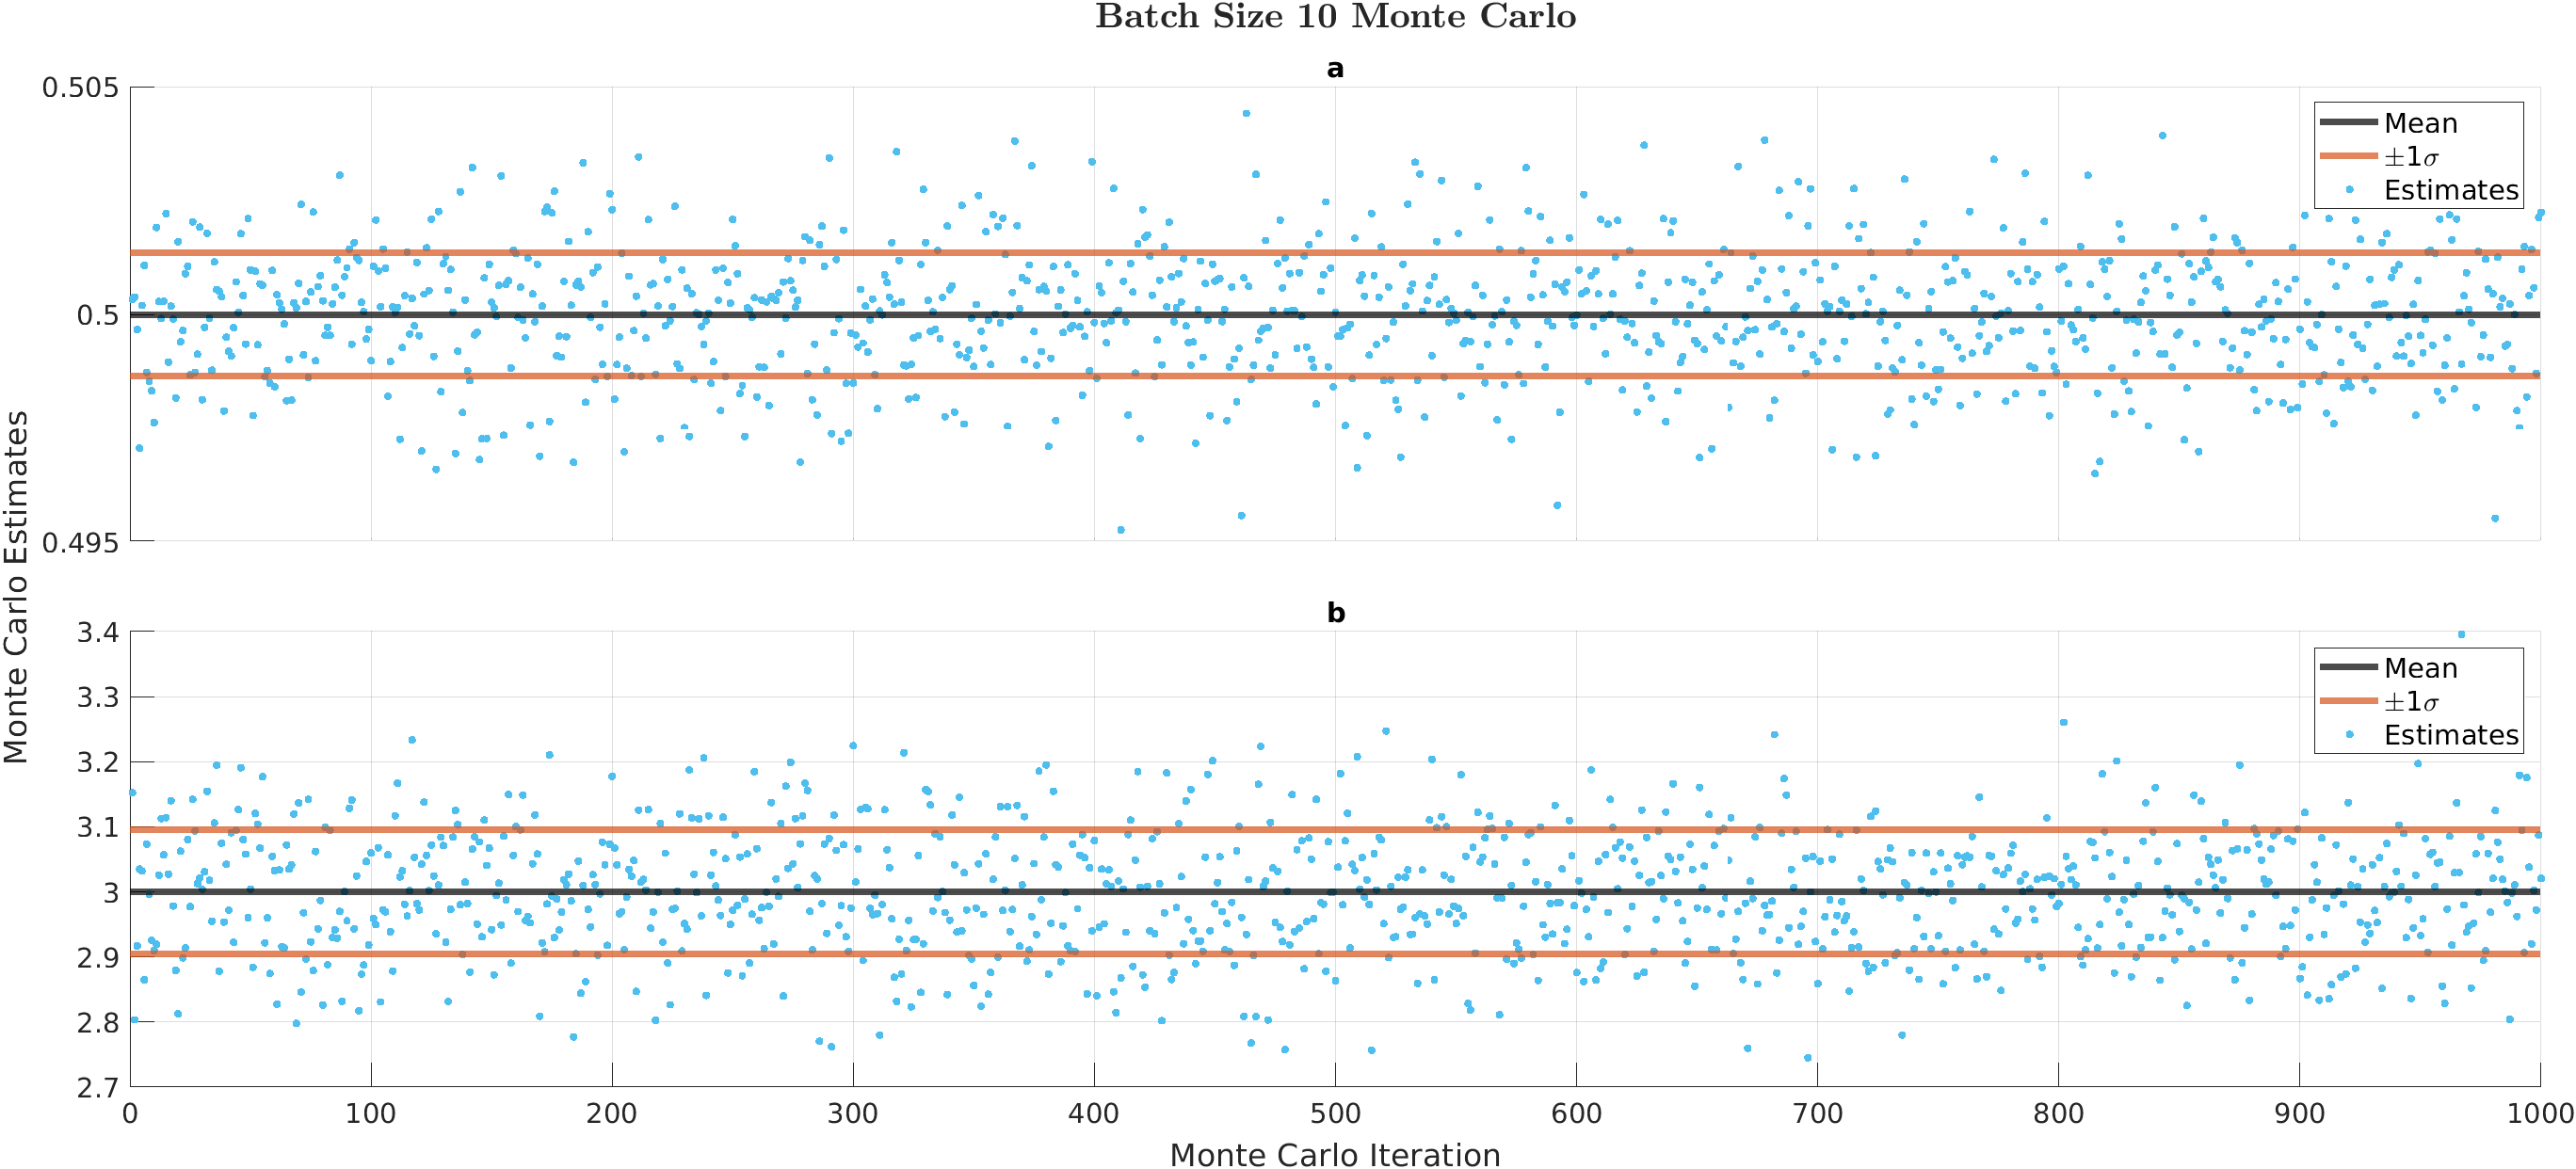
\includegraphics[width=0.85\textwidth]{3b.png}
    \caption{Monte Carlo with batch size of 10.}
  \end{figure}
  Where the theoretical standard deviation values were calculated from the 
  covariance matrix as follows:
  \begin{equation*}
    \begin{split}
      P &= \sigma^2 (H^TH)^{-1} = 0.3^2 (H^TH)^{-1} \\
      \sigma_{theoretical} &= 
      \begin{bmatrix}
        \sqrt{P(1,1)} & \sqrt{P(2,2)}
      \end{bmatrix}^T
      \end{split}
  \end{equation*}
  \begin{figure}[H]
    \centering
    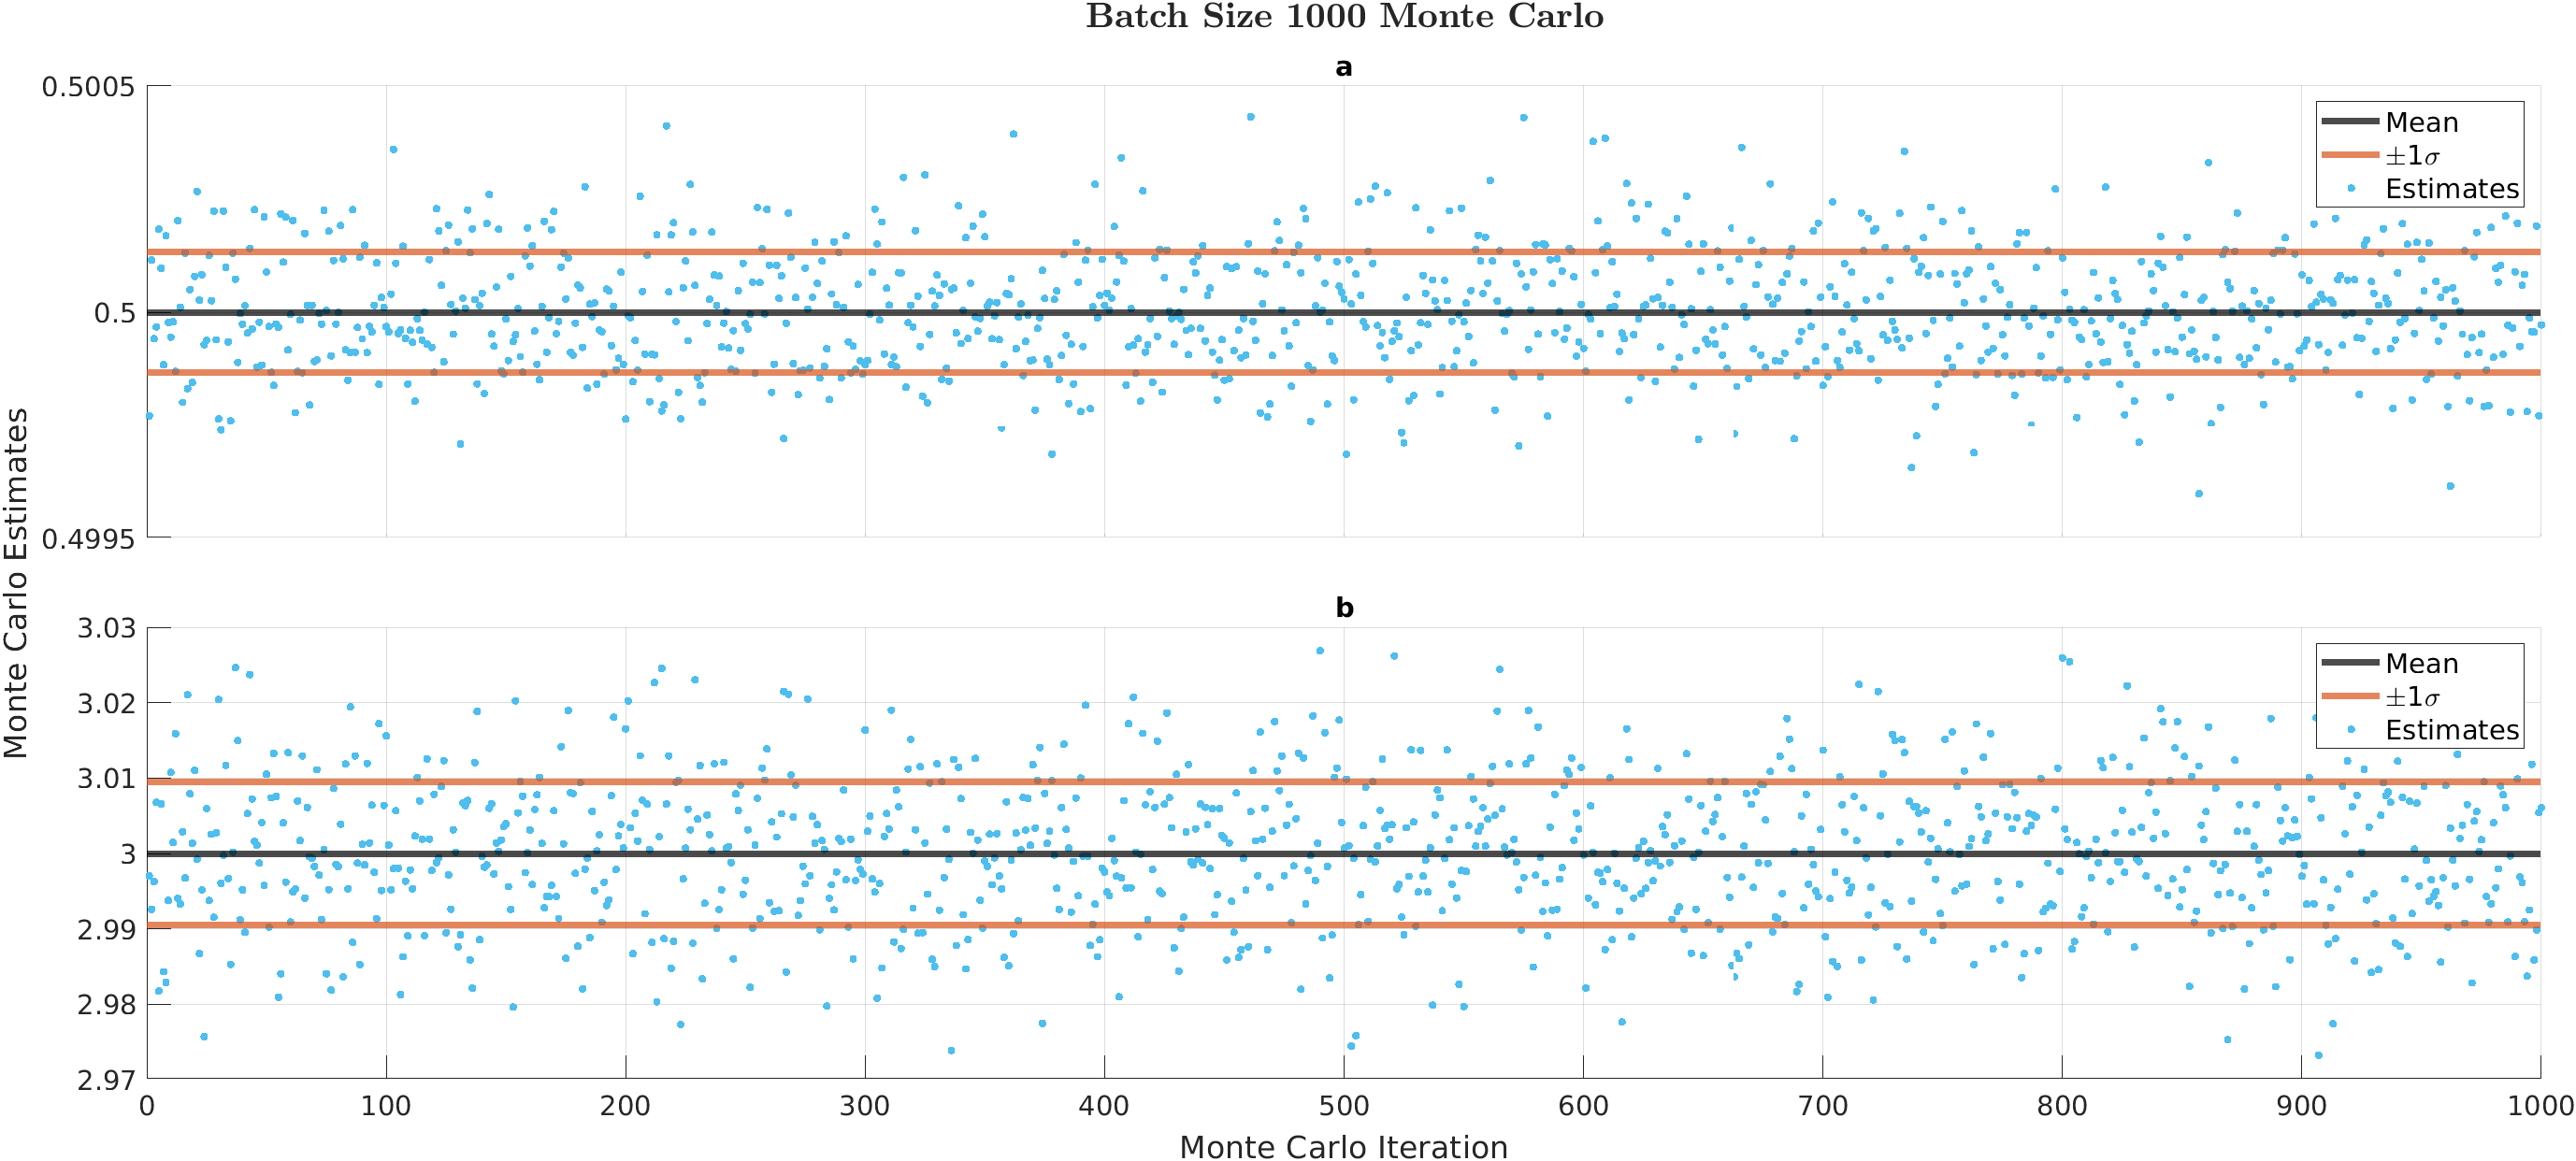
\includegraphics[width=0.85\textwidth]{3c.png}
    \caption{Monte Carlo with batch size of 1000.}
  \end{figure}
  Looking at the above values, the estimates are extremely close the the 
  expected values, with all of the values for $a$ being closer together than 
  the values for $b$. Repeating the monte carlo simulation with a batch size 
  of 1000:
  \begin{equation*}
    \begin{split}
      \sigma_{estimates} = \begin{bmatrix} 0.000131 & 0.009683 \end{bmatrix}^T \\
      \mu_{estimates} = \begin{bmatrix} 0.500000 & 3.000223 \end{bmatrix}^T \\
      \sigma_{theoretical} = \begin{bmatrix} 0.000134 & 0.009487 \end{bmatrix}^T \\
      \mu_{theoretical} = \begin{bmatrix} 0.500000 & 3.000000 \end{bmatrix}^T \\
    \end{split}
  \end{equation*}
  Comparing these estimates to the estimates of a batch size of 10, it is first 
  notable that the estimate mean error decreases as well as the standard 
  deviations converging towards 0. Both decrease by approximately a factor of 
  10 (notice the scale on each plot). \\
  Converting the problem into a recursive least squares setup instead of 
  batched least squares required the following equation adjustments:
  \begin{equation*}
    \begin{split}\
      Q_{k} &= Q_{k-1} + H_k^TH_k \\
      \partial{x} &= Q_k^{-1} H_k^T \left(y_k - H_k x_{k-1}\right) \\
      x_k &= x_{k-1} + \partial{x}
    \end{split}
  \end{equation*}
  This was implemented in MATLAB with the following code for 100 iterations
  between 0 and 1 second:
  \begin{lstlisting}
  dt = 1/100;
  t = (dt:dt:1)';
  R = (0.3^2 * eye(1))^-1;
  x = zeros(2,100);
  P = zeros(2,2,100);
  
  for i = 1:100
      if i == 1
          y = g(t(1));
          H = G(t(1));
          Q = H'*H;
          x(:,1) = Q^-1 * (H'*y);
          P(:,:,1) = 0.3^2 * Q^-1;
      else
          y = g(t(i));
          H = G(t(i));
          Q = Q + H'*H;
          dx = Q^-1 * H' * (y - H*x(:,i-1));
  
          x(:,i) = x(:,i-1) + dx;
          P(:,:,i) = 0.3^2 * Q^-1;
      end
  end
  \end{lstlisting}
  \begin{figure}[H]
    \centering
    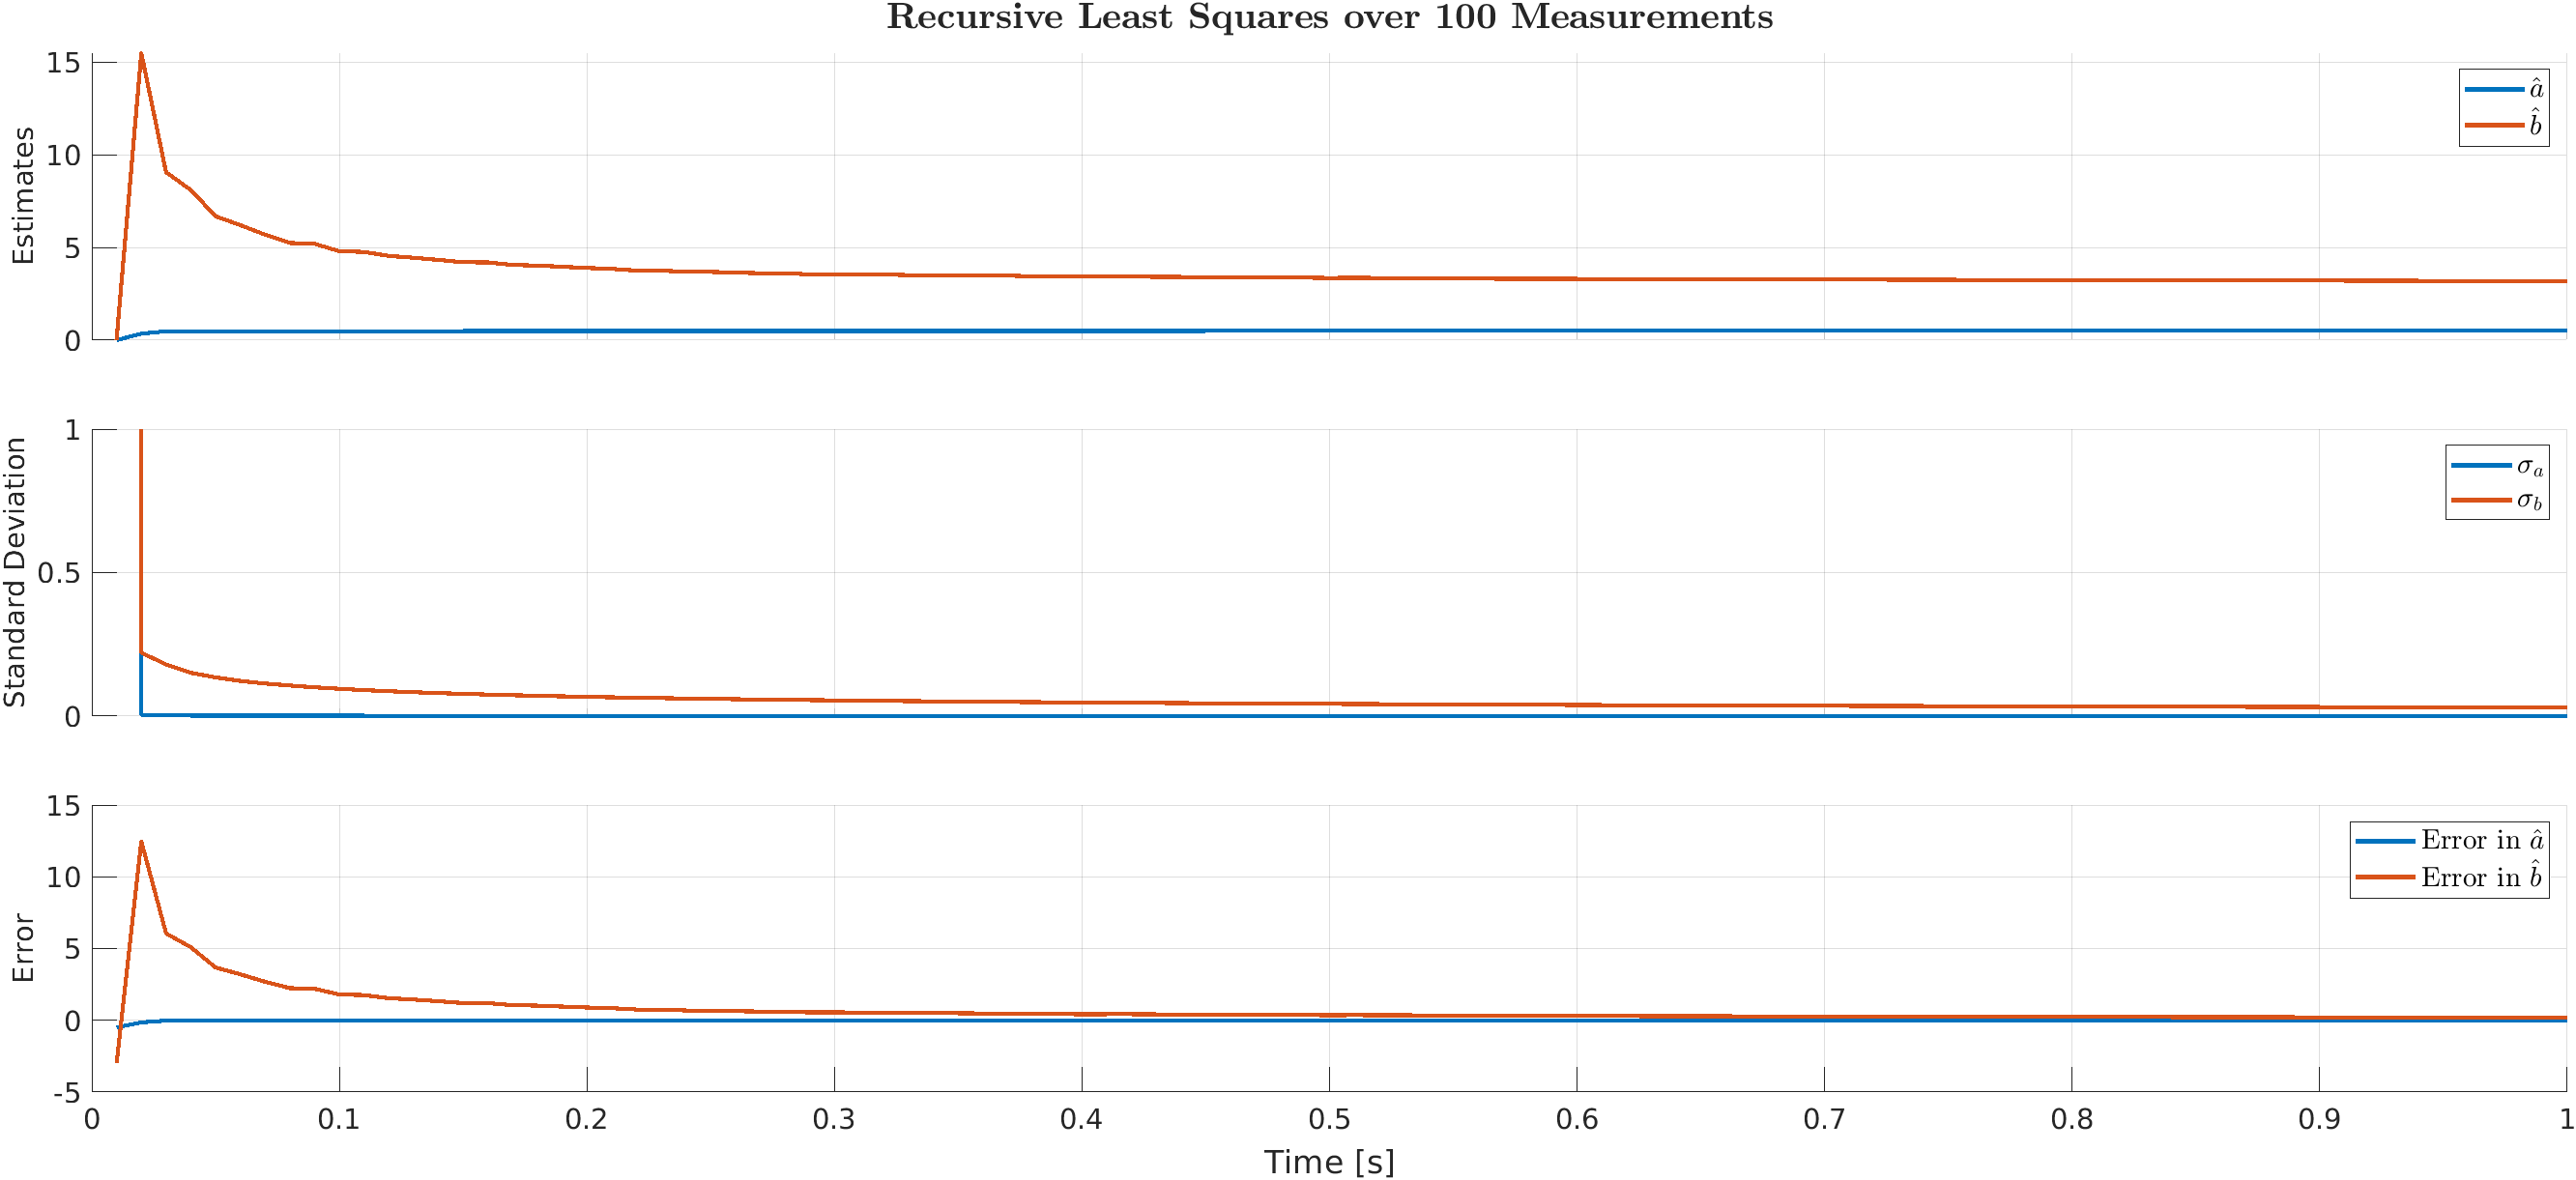
\includegraphics[width=0.85\textwidth]{3d.png}
    \caption{Recursive Least Squares over Time.}
  \end{figure}
  As shown, the first iteration results in a poor solution with a huge standard 
  deviation on the scale of $10^7$ (the axis was scaled to between 0 and 1). 
  After the second iteration, the standard deviation reduces to more 
  reasonable values, and by the end of the run, the estimates have 
  converged to approximately the correct values.

  % PROBLEM 4
  \newpage
  \item Least Squares for System I.D.  Simulate the following discrete system 
  with a normal random input and output noise:
  \begin{equation*}
    G(z) = \dfrac{0.25(z-0.8)}{z^2-1.90z+0.95}
  \end{equation*}
  \begin{enumerate}[(a)]
    \item Develop the H matrix for the least squares solution.
    \item Use least squares to estimate the coefficients of the above 
    Transfer Function. How good is the fit?  Plot the bode response of the 
    I.D. TF and the simulated TF on the same plot. How much relative noise 
    has been added (SNR - signal to noise ratio), plot y and Y on the same 
    plot.
    \item Repeat the estimation process about 10 times using new values for 
    the noise vector each time. Compute the mean and standard deviation of 
    your parameter estimates. Compare the computed values of the parameter 
    statistics with those predicted by the theory based on the known value of 
    the noise statistics.
    \item Now use sigma between 0.1 and 1.0 and repeat parts b and c.
    \item What can you conclude about using least squares for system id with 
    large amounts of noise?
  \end{enumerate}
  \solution
  To develop a geometry matrix for the system, the transfer function is 
  generalized to the following:
  \begin{equation*}
    \dfrac{Y}{U} = \dfrac{az + b}{z^2 + cz + d}
  \end{equation*}
  Expanding and performing an inverse z-transform with U defined as the input 
  and Y defined as the output:
  \begin{equation*}
    \begin{split}
      U(az+ b) &= Y(z^2 + cz + d) \\
      aU_{k+1} + bU_{k} &= Y_{k+2} + cY_{k+1} + dY_{k}
    \end{split}
  \end{equation*}
  Taking $Y_{k+2}$ as the measurements of the system, the geometry matrix can 
  be defined as follows:
  \begin{equation*}
    H = 
    \begin{bmatrix}
      U_{k+1} & U_{k} & -Y_{k+1} & -Y_{k}
    \end{bmatrix}
  \end{equation*}
  And the full system.
  \begin{equation*}
    Y_{k+2} = 
    \begin{bmatrix}
      U_{k+1} & U_{k} & -Y_{k+1} & -Y_{k}
    \end{bmatrix}
    \begin{bmatrix}
      a \\ b \\ c \\ d
    \end{bmatrix}
  \end{equation*}
  Using the following MATLAB code to estimate the coefficients:
  \begin{lstlisting}
  % discrete system
  num = 0.25 .* [1, -0.8]; 
  den = [1, -1.9, 0.95];
  G = tf(num,den, 1);
  
  % simulated discrete system
  U = randn(1000,1);
  y = dlsim(num,den,U); 
  sigma = 0.01;
  Y = y + sigma*randn(1000,1); 
  
  % least squares coefficient estimation
  H = [U(2:end-1), U(1:end-2), -Y(2:end-1), -Y(1:end-2)];
  m = Y(3:end);
  x = (H'*H)^-1*H'*m;
  P = sigma^2 * (H'*H)^-1;
  
  % recreated system
  numid = [x(1), x(2)];
  denid = [1, x(3), x(4)];
  Gid = tf(numid,denid, 1);
  SNR = std(Y) / sigma;
  \end{lstlisting}
  Resulting in the following bode plot and signal plot.
  \begin{figure}[H]
    \centering
    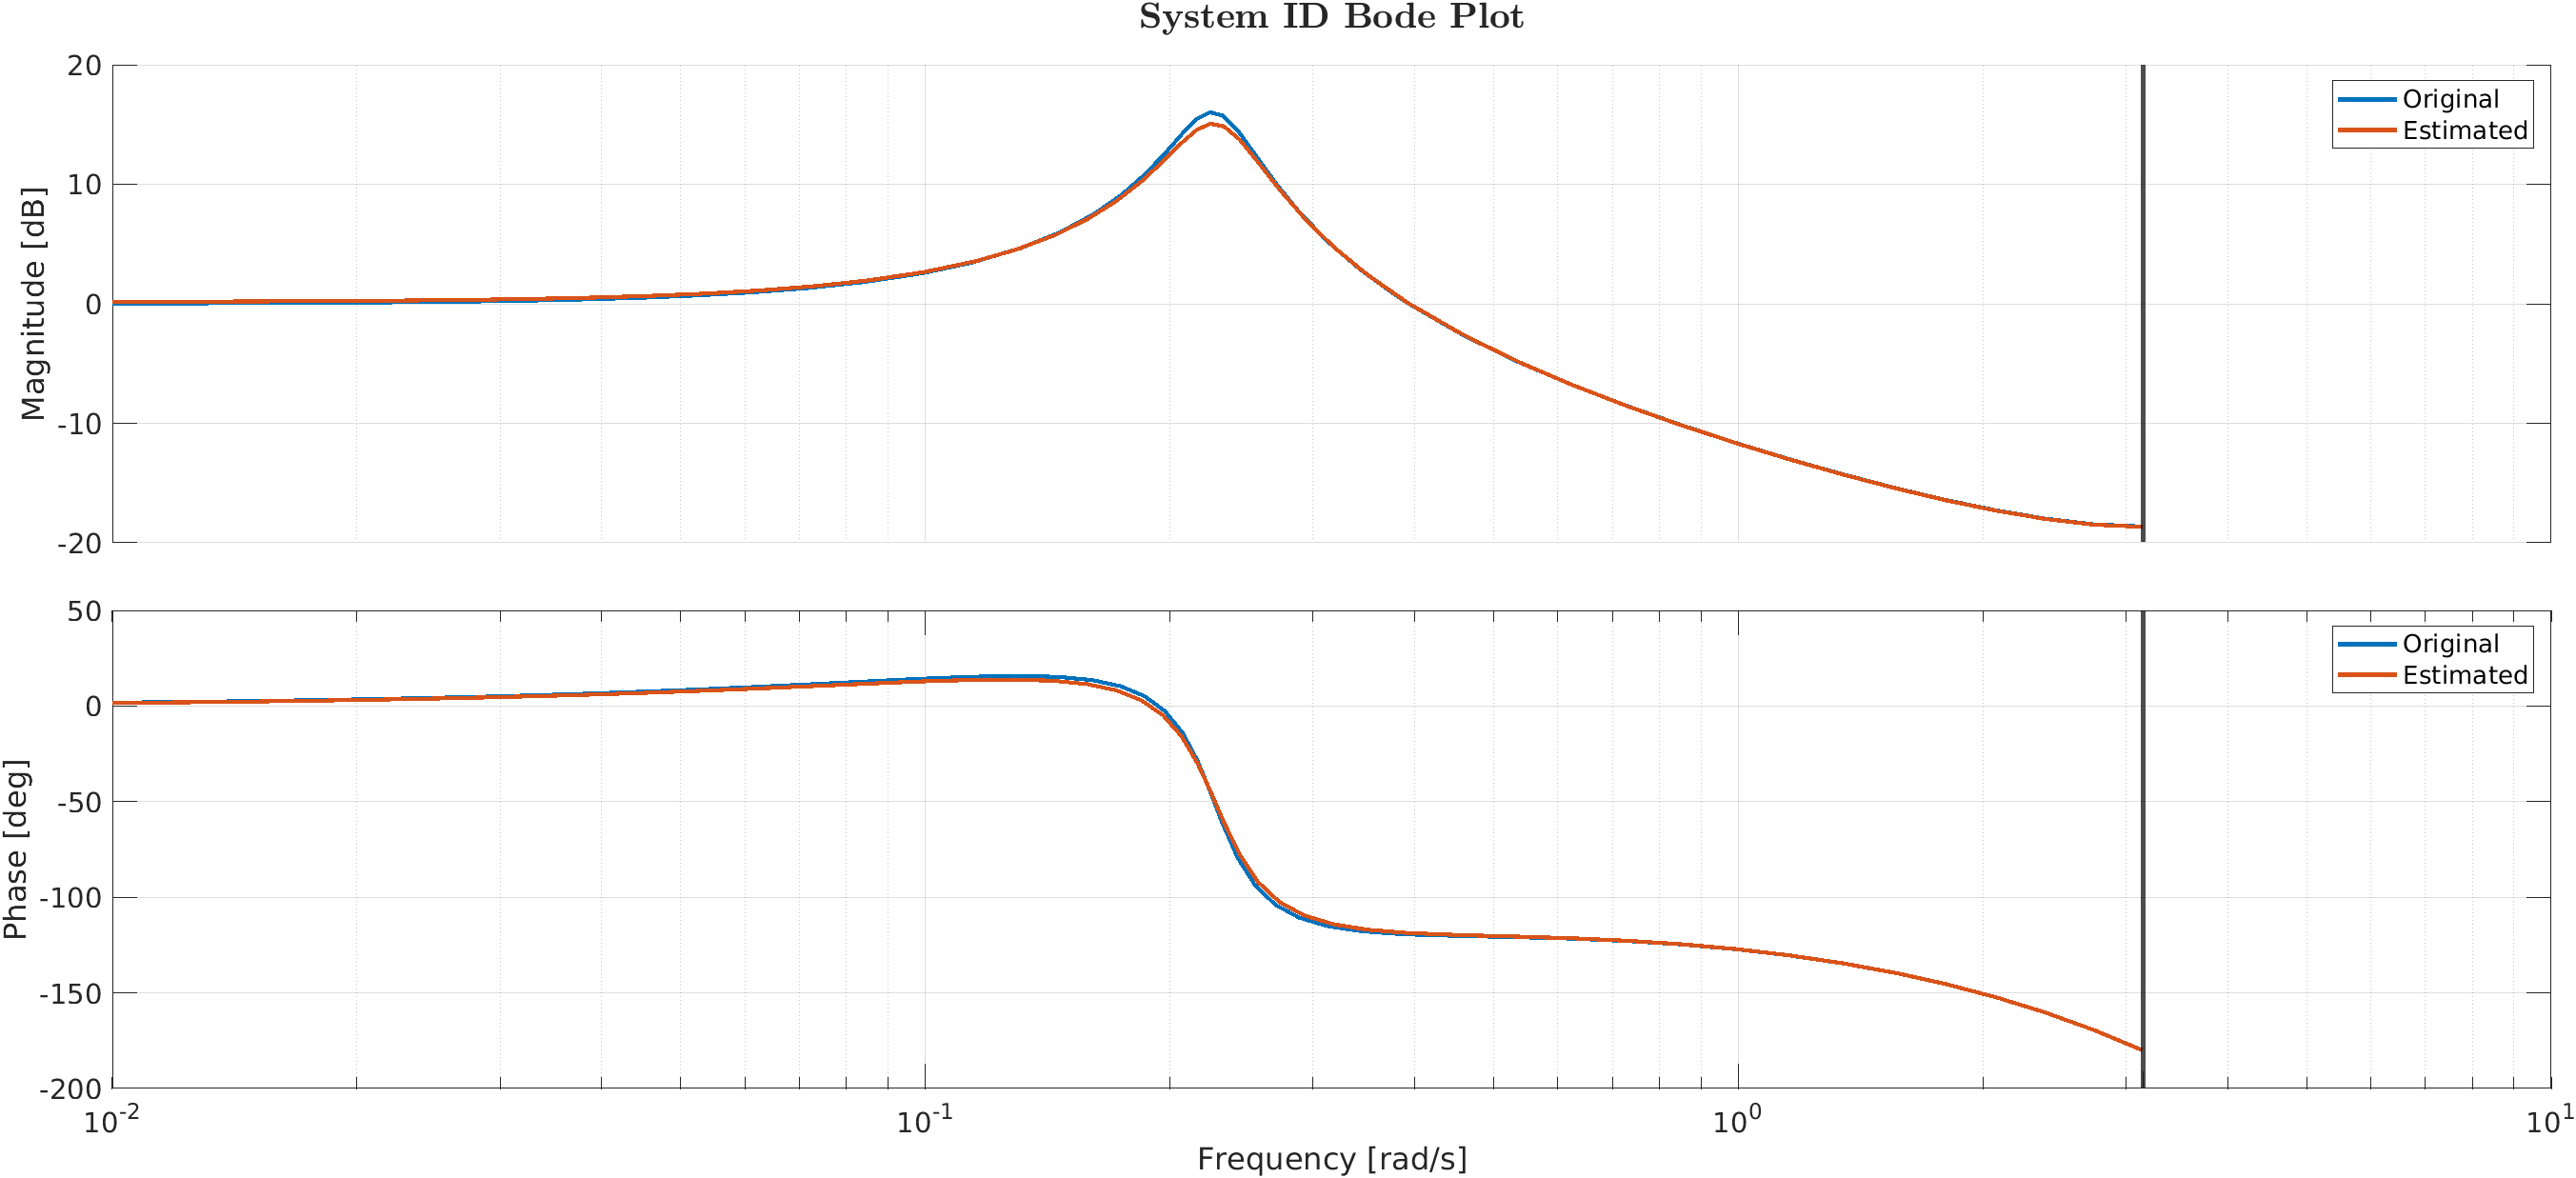
\includegraphics[width=0.85\textwidth]{4b.png}
    \caption{Bode Plot of Simulated and I.D. System.}
  \end{figure}
  \begin{figure}[H]
    \centering
    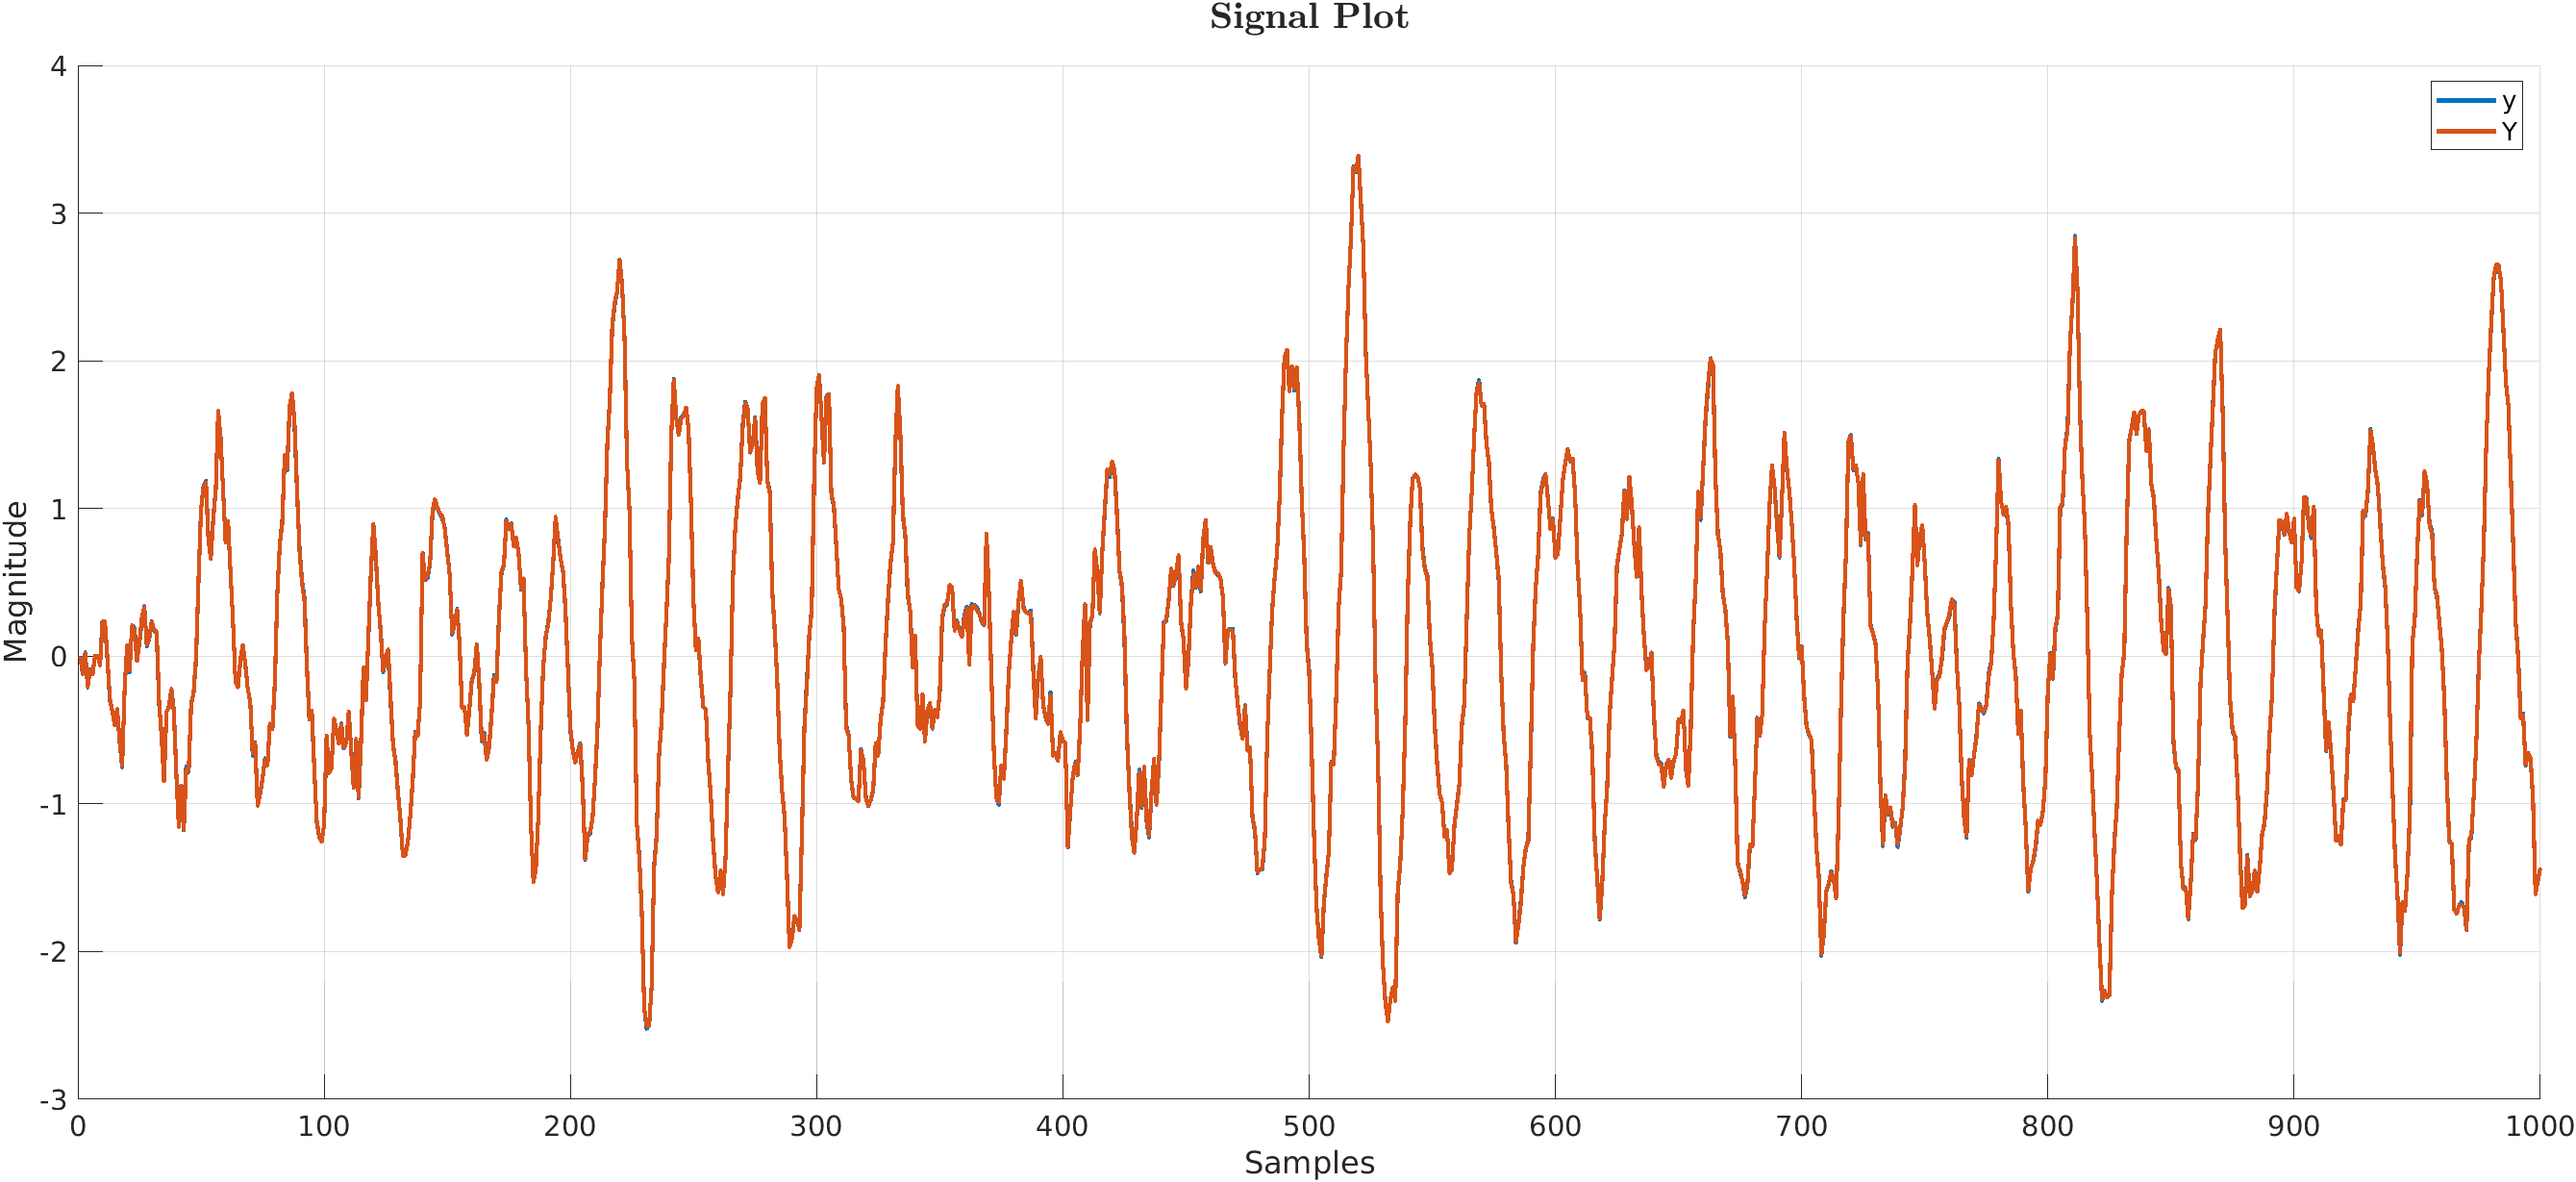
\includegraphics[width=0.85\textwidth]{4b-1.png}
    \caption{Simulated and Recreated Signal.}
  \end{figure}
  As shown, the recreated system is almost exactly the same as the original due 
  to the small amount of noise added to the signal. The calculated estimates and 
  signal to noise ratio were:
  \begin{equation*}
    \begin{split}
      x &= \begin{bmatrix} 0.251377 & -0.199053 & -1.892648 & 0.942921 \end{bmatrix}^T \\
      SNR &= 95.299670
    \end{split}
  \end{equation*}
  Running a 10 iteration monte carlo to get an idea of the system statistics:
  \begin{equation*}
    \begin{split}
      \sigma_{estimated} &= \begin{bmatrix} 0.000817 & 0.001139 & 0.001296 & 0.001205 \end{bmatrix}^T \\
      \mu_{estimated} &= \begin{bmatrix} 0.249995 & -0.197918 & -1.892480 & 0.942775 \end{bmatrix}^T \\
      \sigma_{theoretical} &= \begin{bmatrix} 0.000315 & 0.000512 & 0.001603 & 0.001554 \end{bmatrix}^T \\
      \mu_{theoretical} &= \begin{bmatrix} 0.250000 & -0.200000 & -1.900000 & 0.950000 \end{bmatrix}^T \\
    \end{split}
  \end{equation*}
  While the means are almost equivalent, the standard deviations are not as close 
  likely due to the small sample size used in the monte carlo simulation. 
  Iterating this monte carlo simulation through a loop of $\sigma$ values 
  between 0.1 and 1 results in the following characteristics:
  \begin{figure}[H]
    \centering
    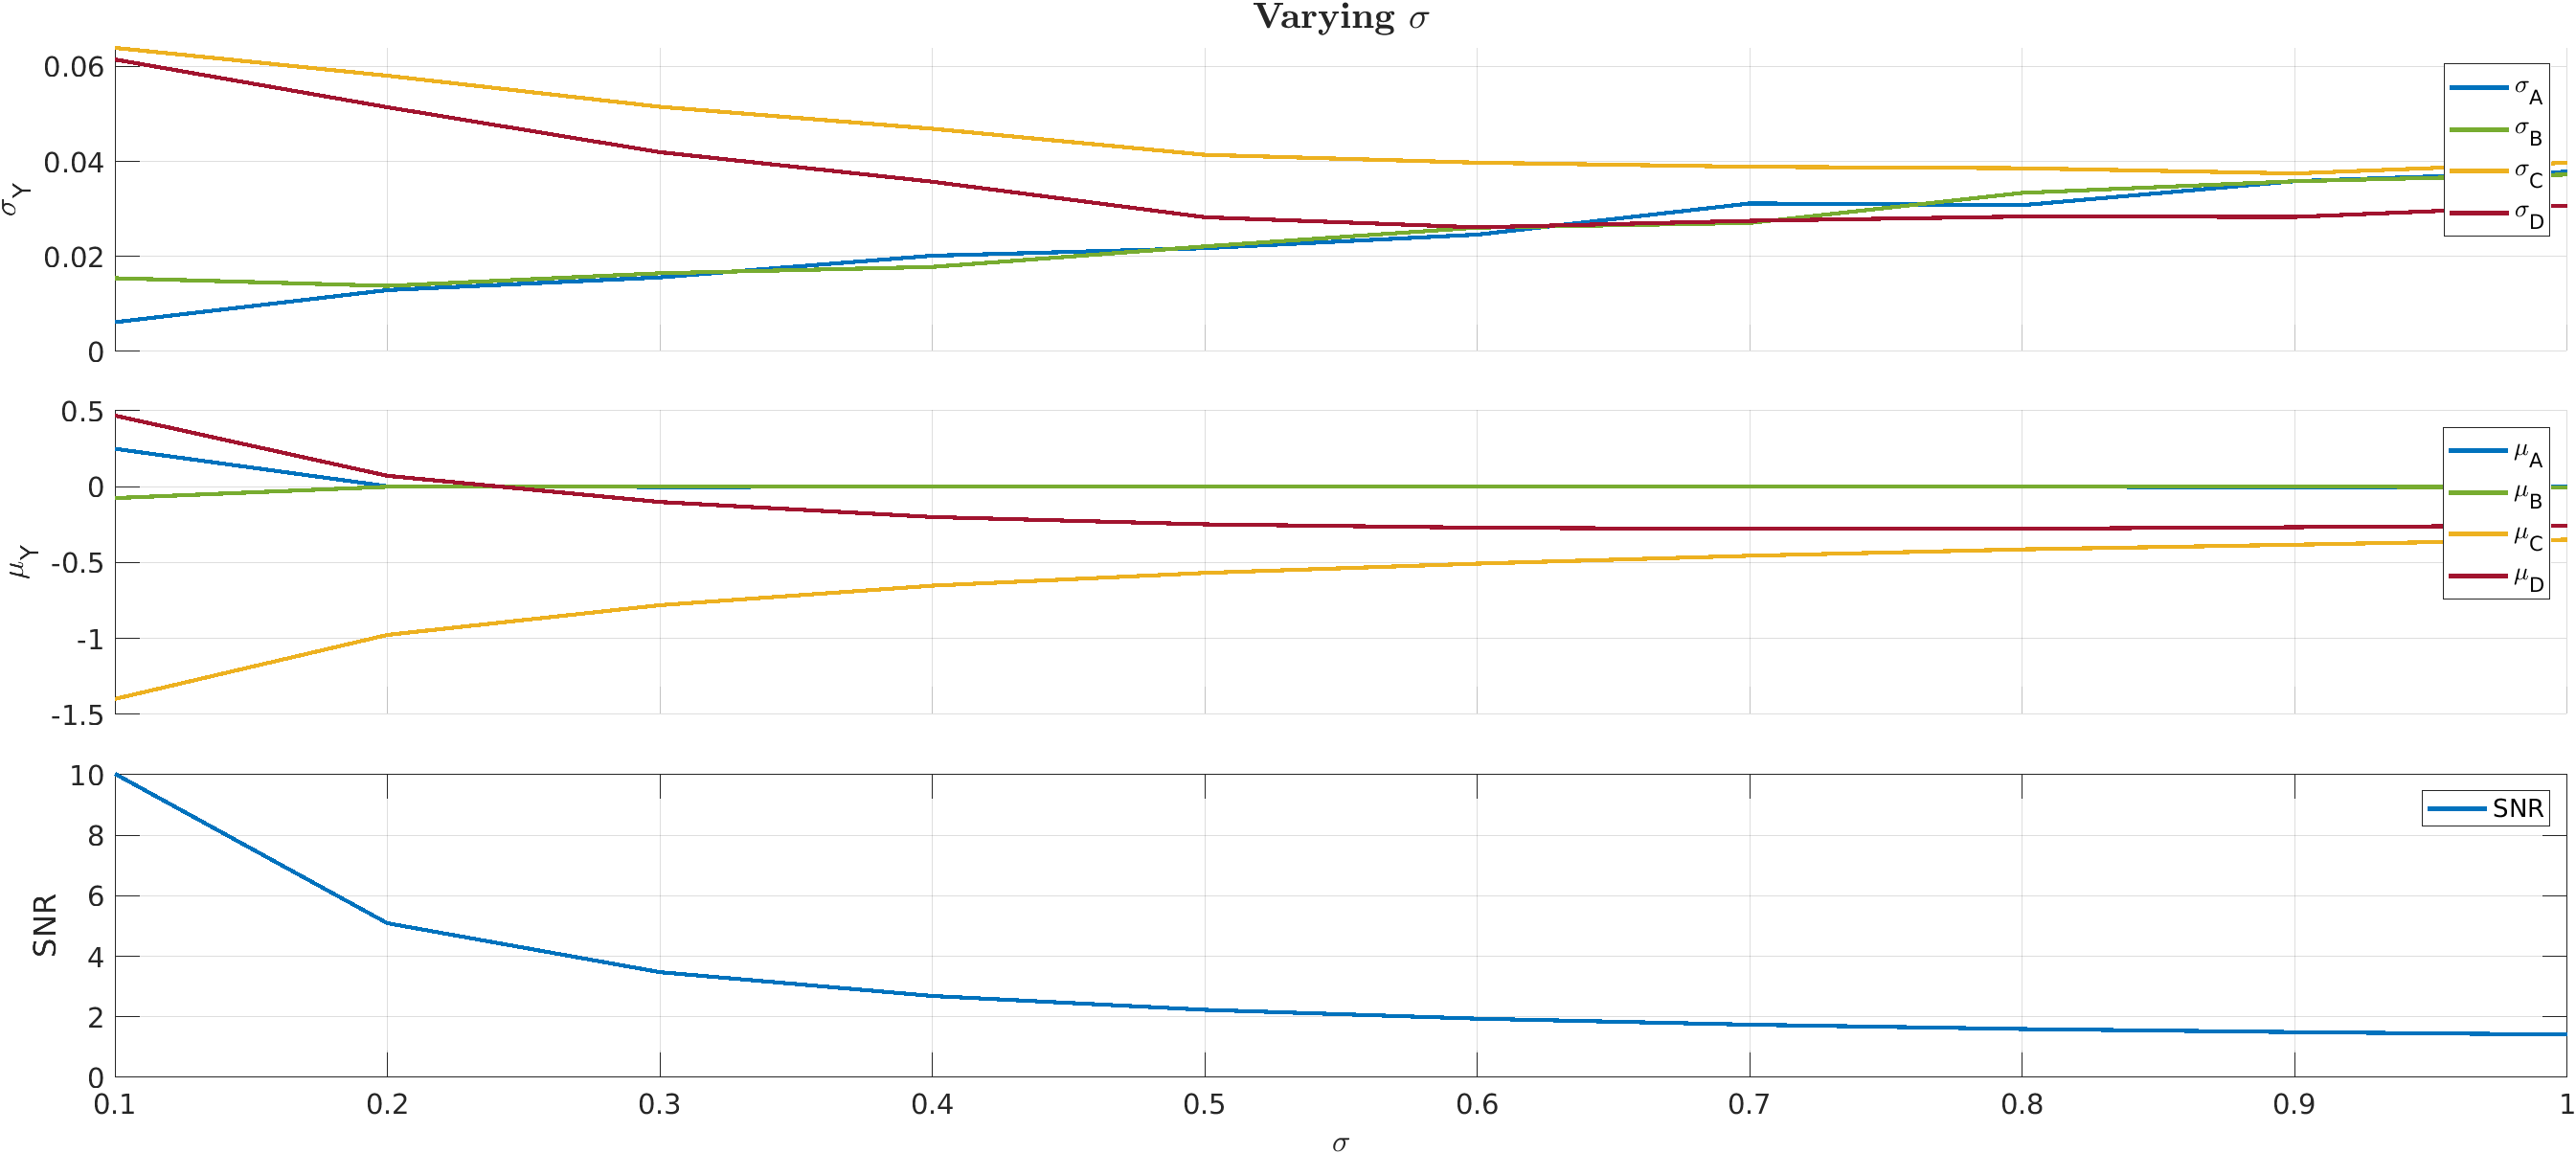
\includegraphics[width=0.85\textwidth]{4d.png}
    \caption{Effects of Higher Noise Levels.}
  \end{figure}
  As displayed, the mean estimates drift far from the actual values and the 
  signal to noise ratio gets extremely low as the recreated signal becomes 
  dominated by the noise. Redoing the bode plot and signal plot for a standard 
  deviation of 1.
  \begin{figure}[H]
    \centering
    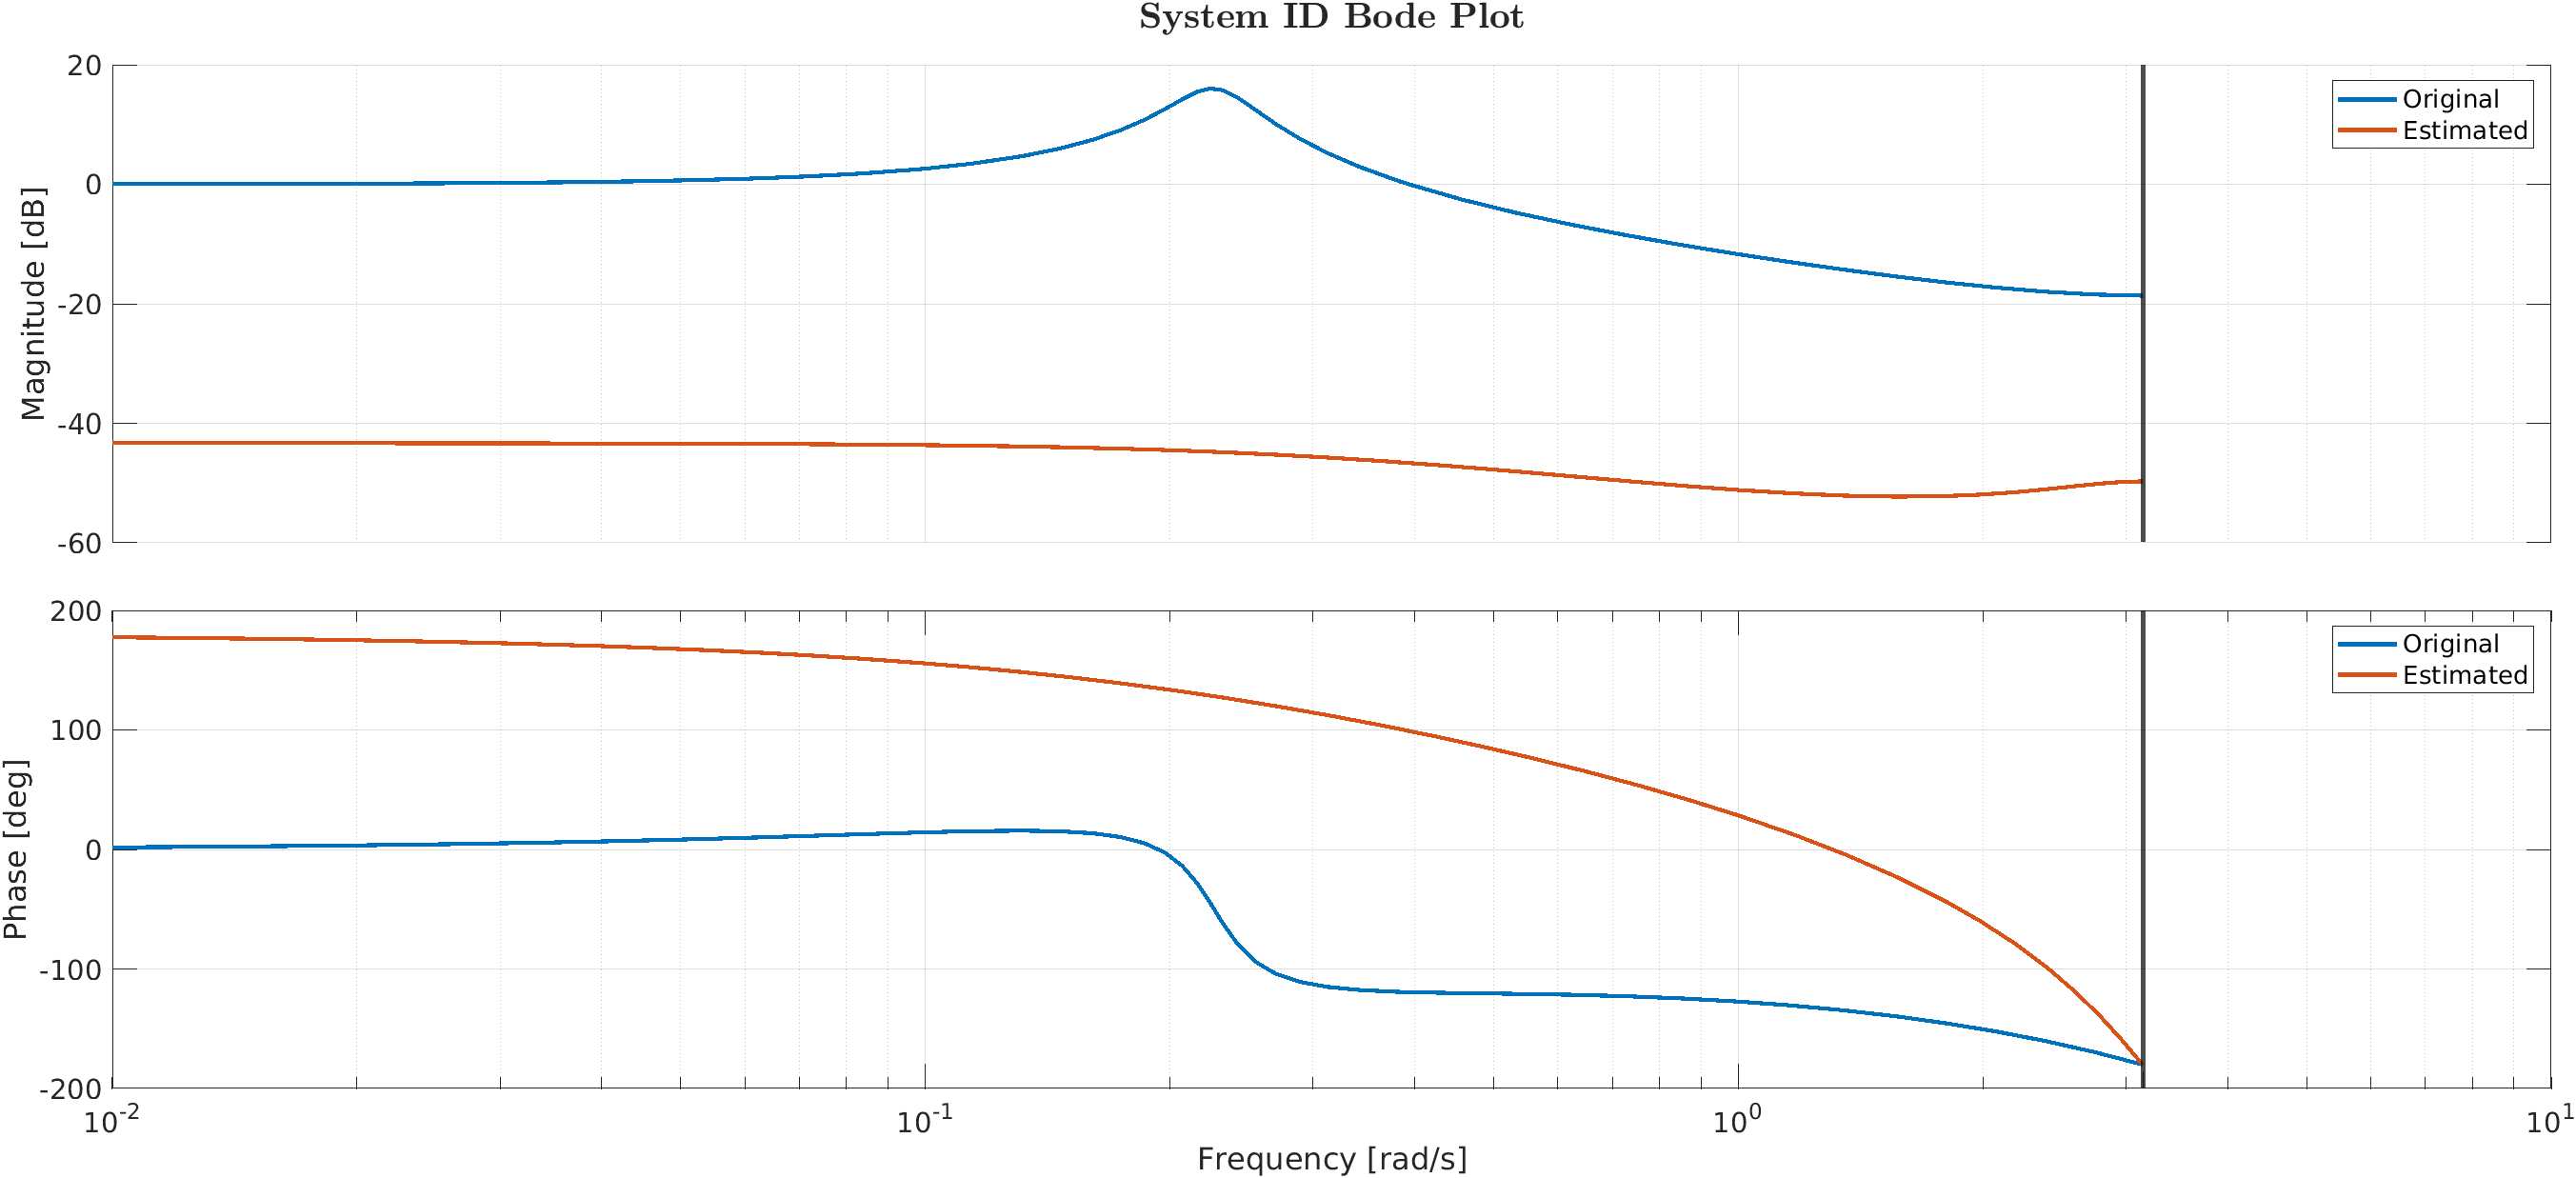
\includegraphics[width=0.85\textwidth]{4e.png}
    \caption{Bode Plot of Simulated and I.D. System with $\sigma=1$.}
  \end{figure}
  \begin{figure}[H]
    \centering
    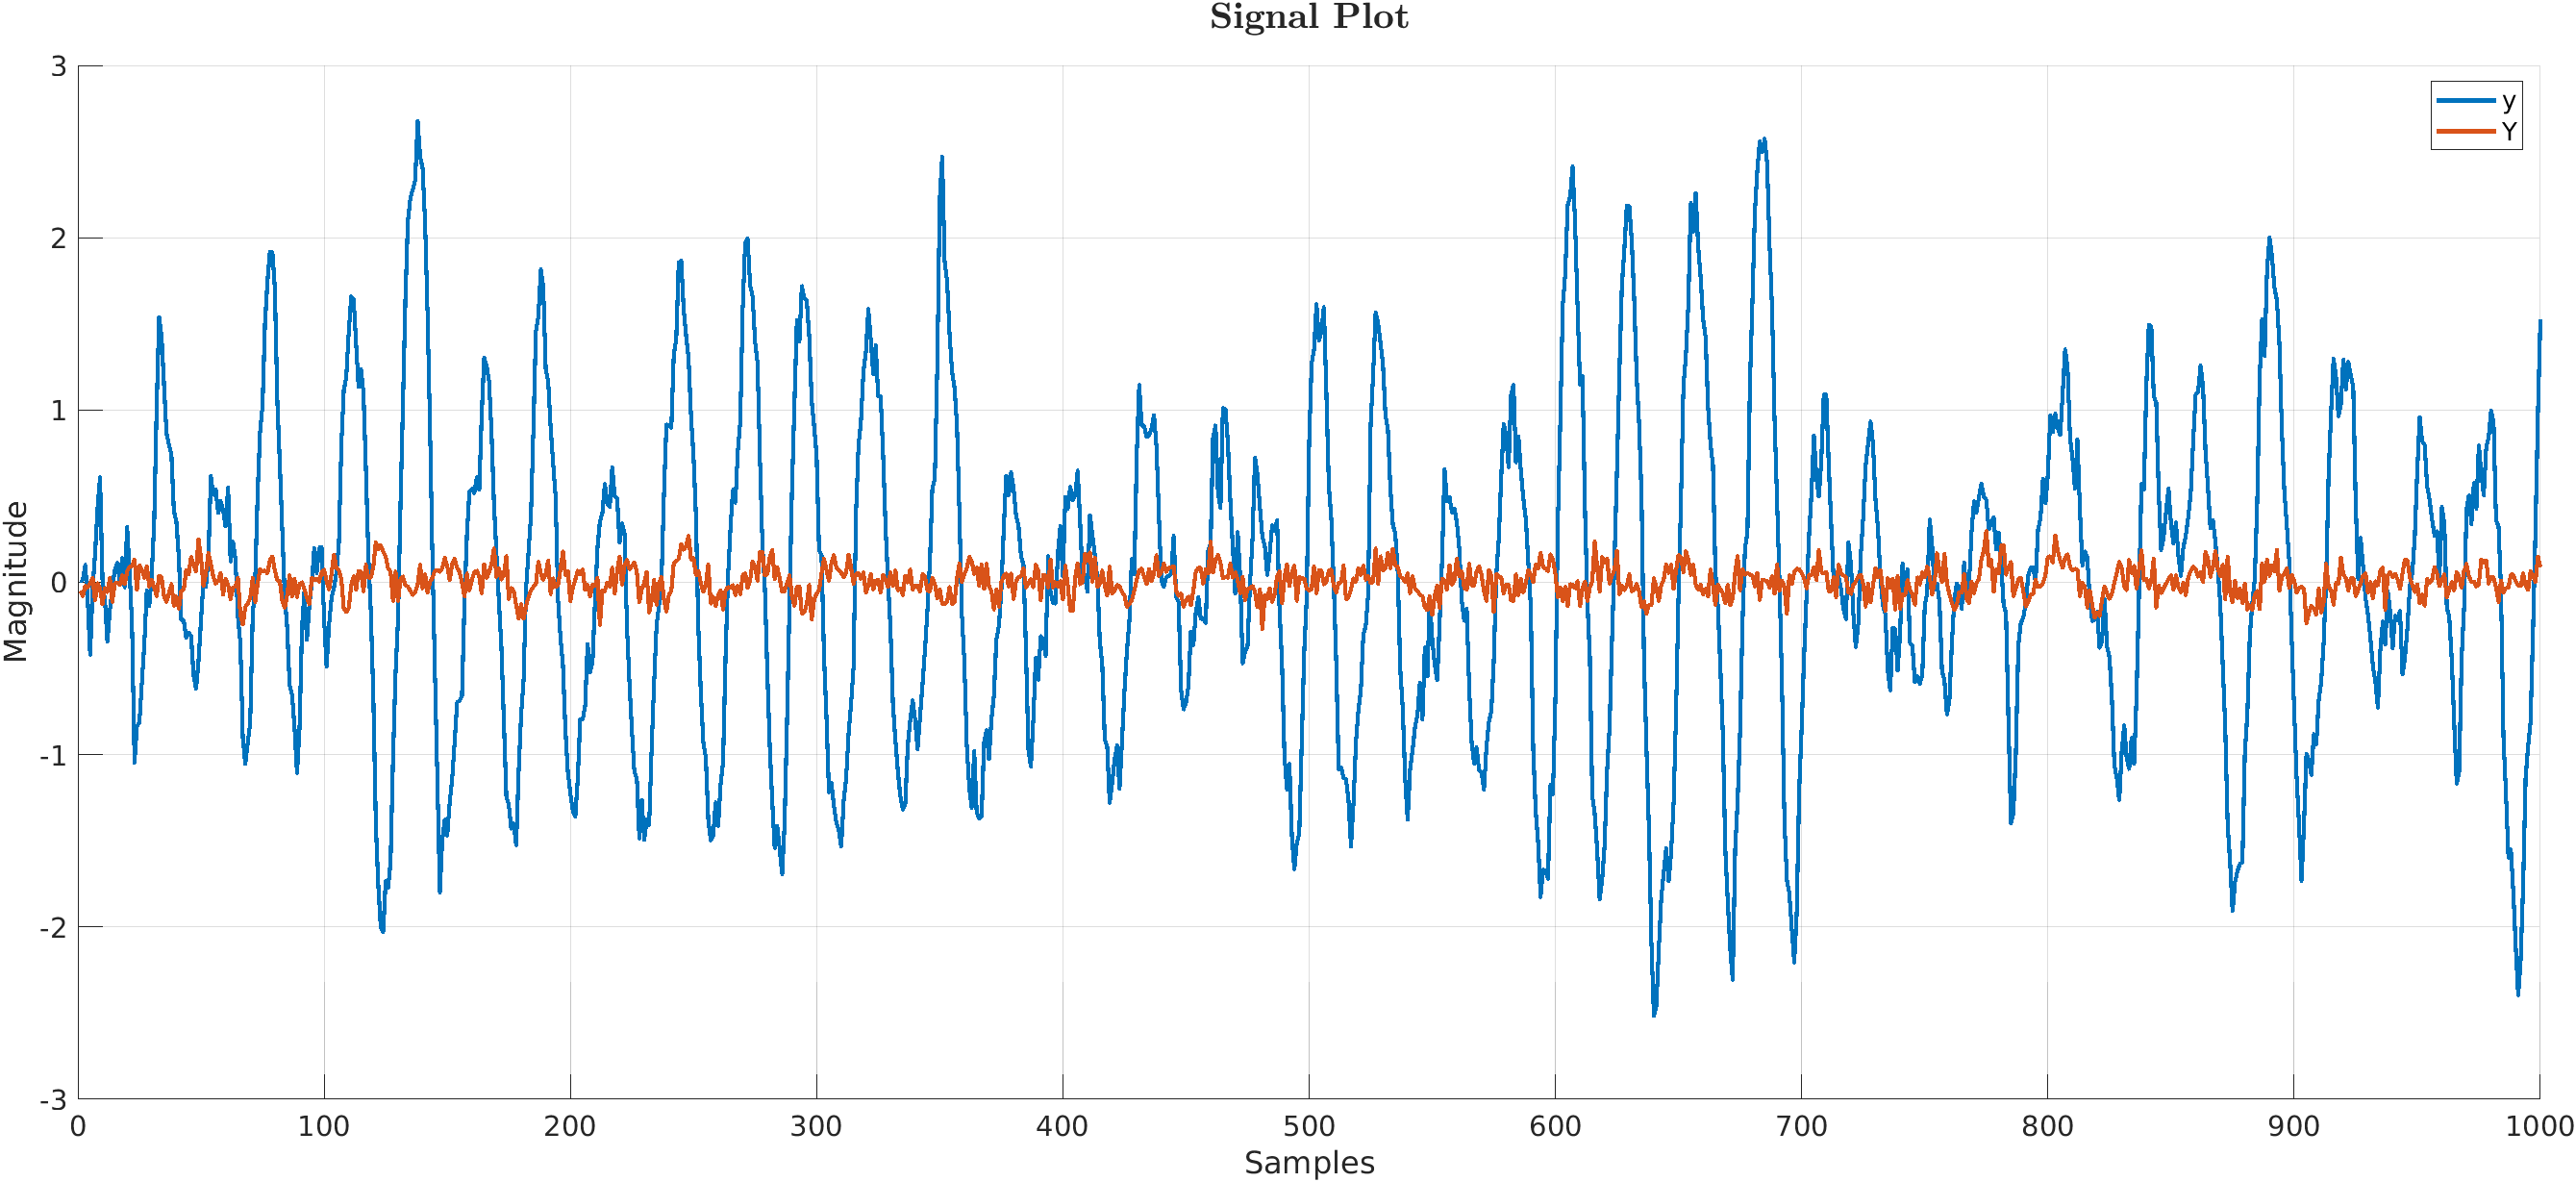
\includegraphics[width=0.85\textwidth]{4e-1.png}
    \caption{Simulated and Recreated Signal with $\sigma=1$.}
  \end{figure}
  As shown the input signal and output signal are completely uncorrelated. This 
  leads to the conclusion that least squares system identification with high 
  noise levels is not plausible as the noise overpowers the fit of the signal.

  % PROBLEM 5
  \vspace{24pt}
  \item Justification of white noise for certain problems. Consider two 
  problems:
  \begin{equation*}
    S_y(j\omega) = |G(j\omega)|^2 S_{\omega}(j\omega)
  \end{equation*}
  \begin{enumerate}[(i)]
    \itemsep -2pt
    \item Simple first order low-pass filter with bandlimited white noise 
    as the input:
    \begin{equation*}
      \begin{split}
        y &= G(s)\omega \:\:\ni\:\: S_y(j\omega)=|G(j\omega)|^2S_{\omega}(j\omega) \\
        S_1(\omega) &= 
        \begin{cases}
          A & \mbox{ } |\omega| \le \omega_c \\
          0 & \mbox{ } |\omega| > \omega_c
        \end{cases} \\
        G(s) &= \dfrac{1}{T_{\omega}s+1}
      \end{split}
    \end{equation*}
    \item The same low pass system, but with pure white noise as the input.
    \begin{equation*}
      \begin{split}
        S_2(\omega) &= A \:\:\forall\:\: \omega \\
        G(s) &= \dfrac{1}{T_{\omega}s+1}
      \end{split}
    \end{equation*}
  \end{enumerate}
  The first case seems quite plausible, but the second case has an input with 
  infinite variance and so is not physically realizable. However, the white 
  noise assumption simplifies the system analysis significantly, so it is 
  important to see if the assumption is justified. We test this with our 
  two examples above: 
  \begin{enumerate}[(a)]
    \itemsep -2pt
    \item Sketch the noise PSD and $|G(j\omega)|$ for a reasonable value of 
    $T_{\omega}$ and $\omega_c$ to compare the two cases. 
    \item Determine the $S_y(j\omega)$ for the two cases.  Sketch these too. 
    \item Determine $E\{y^2\}$ for the two cases.
    \item Use these results to justify the following statement:
    "If the input spectrum is flat considerably beyond the system bandwidth, 
    there is little error introduced by assuming that the input spectrum is 
    flat out to infinity."
  \end{enumerate}
  \solution
  Sketching the plots for of the input PSD of band-limited white noise, pure white noise, 
  and the bode plot of the transfer function.
  \begin{figure}[H]
    \centering
    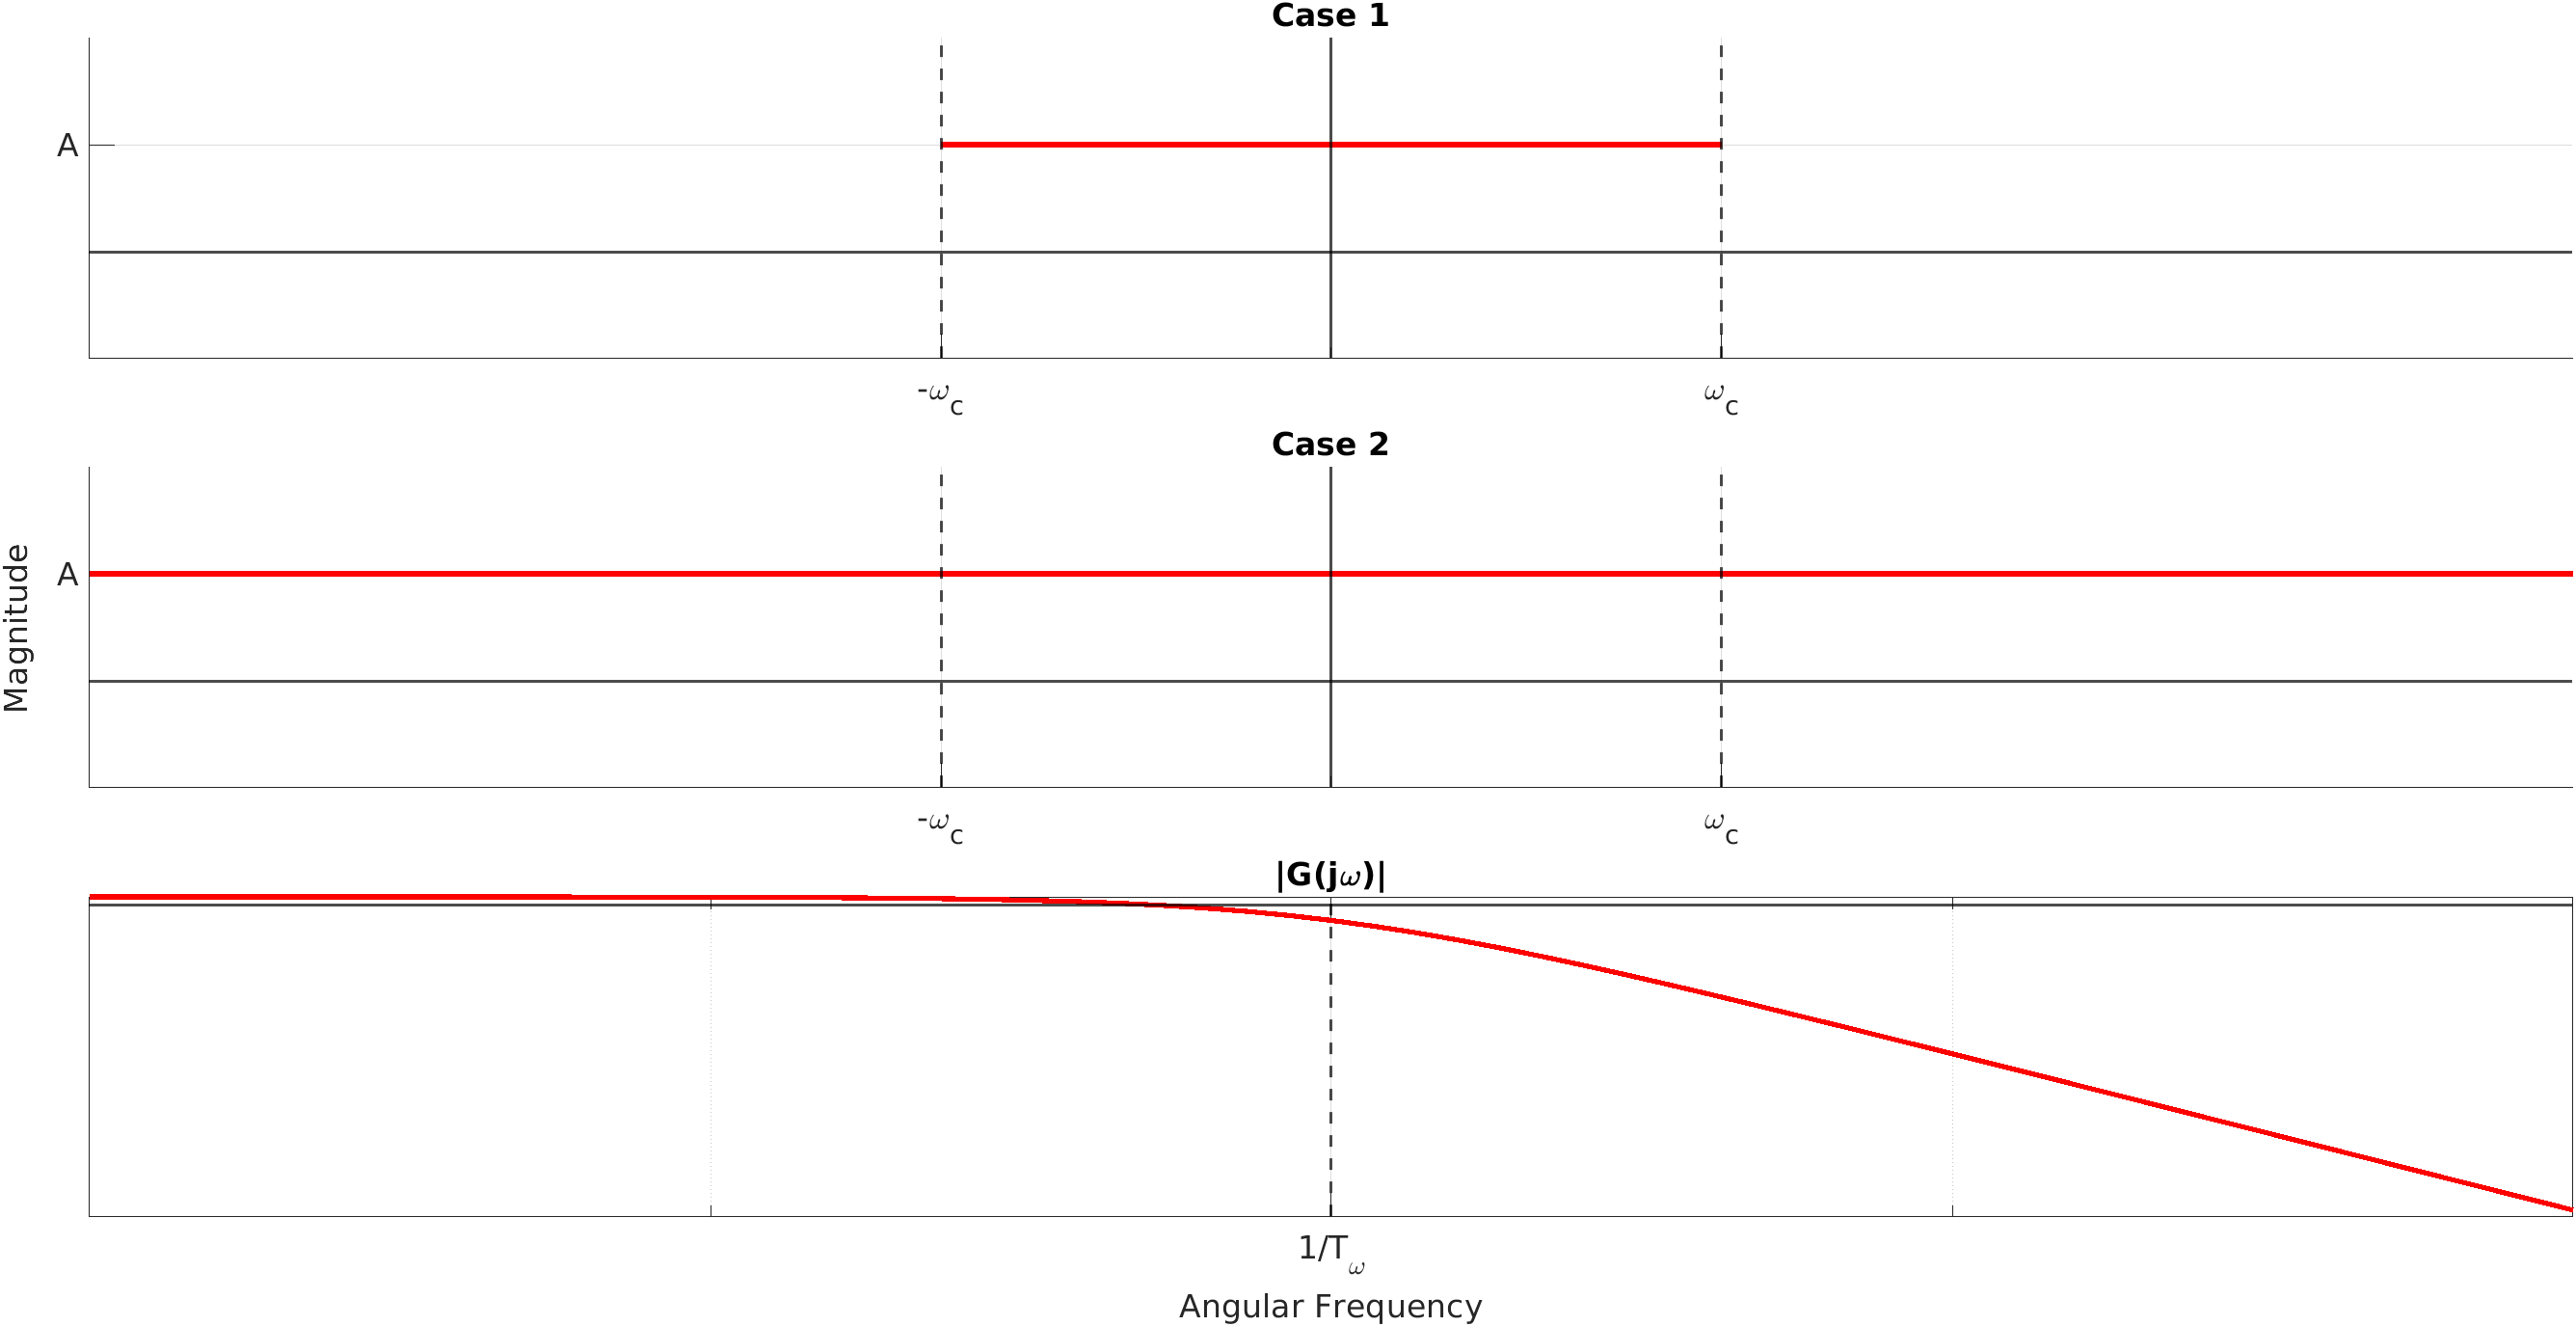
\includegraphics[width=0.85\textwidth]{5a.png}
    \caption{Drawings of the Input PSDs.}
  \end{figure}
  To determine the PSD of the output using the given equation:
  \begin{equation*}
    \begin{split}
      S_y(j\omega) &= |G(j\omega)|^2 S_{\omega}(j\omega) \\
      &= \biggr| \dfrac{1}{T_{\omega}(j\omega) + 1} \biggr|^2 S_{1|2}(\omega) \\
      &= \dfrac{1}{T_{\omega}^2 \omega^2 + 1} S_{1|2}(\omega) \\
    \end{split}
  \end{equation*}
  For case 1, $S_{1|2} = A$ between $-\omega_c \le \omega \le \omega_c$ and for case 
  2, $S_{1|2} = A$ is always $A$. Sketching the two output PSDs. 
  \begin{figure}[H]
    \centering
    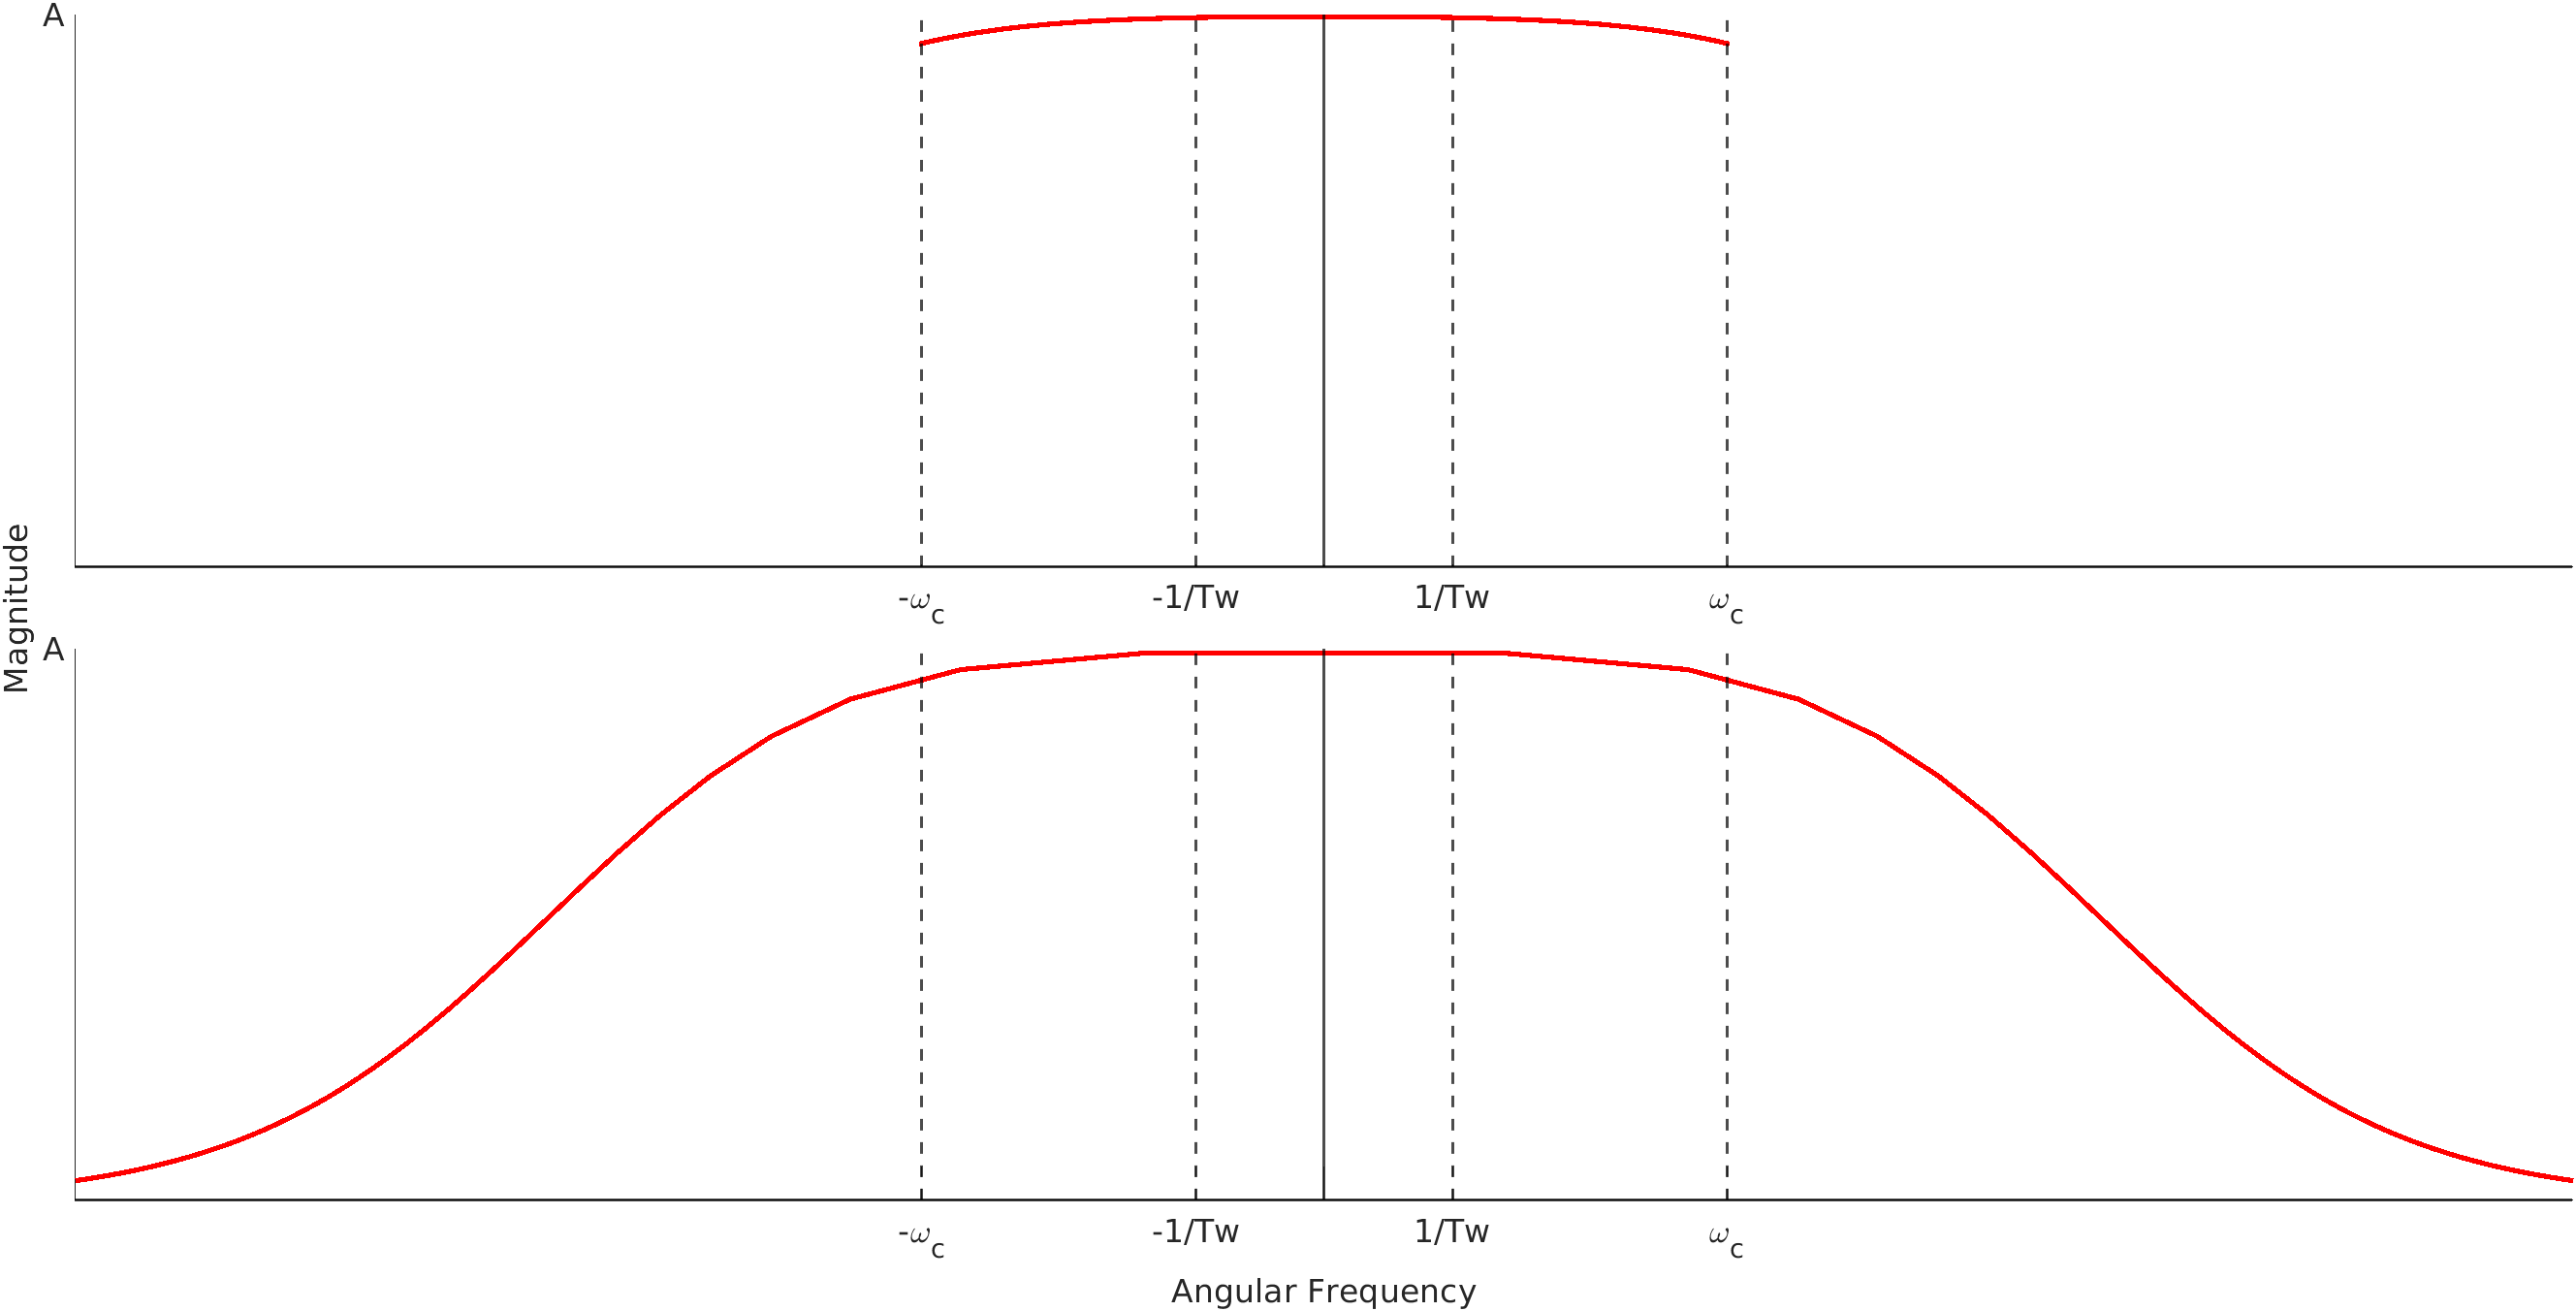
\includegraphics[width=0.85\textwidth]{5b.png}
    \caption{Drawings of the Output PSDs.}
  \end{figure}
  To determine $E\{y^2\}$, the integral of the PSD can be taken. Since white noise 
  has a mean of 0 and is uncorrelated with itself, this expectation is equivalent 
  to the variance.
  \begin{equation*}
    \begin{split}
      E\{y^2 - \bar{y}^2\} &= E\{y^2\} - E\{\bar{y}^2\} = E\{y^2\} - 0 \\
      &= E\{y^2\} \\
      &= \int S_y(j\omega) d\omega
    \end{split}
  \end{equation*}
  For case 1:
  \begin{equation*}
    \begin{split}
      E\{y^2\} &= \int_{-\omega_c}^{\omega_c} \dfrac{1}{T_{\omega}^2 \omega^2 + 1} A d\omega \\
      &= \dfrac{A}{T_{\omega}} \tan^{-1}(T_{\omega}\omega) \biggr|_{-\omega_c}^{\omega_c} \\
      &= \dfrac{A}{T_{\omega}} \left( \tan^{-1}(T_{\omega}\omega_c) - \tan^{-1}(-T_{\omega}\omega_c) \right) \\
      &= \dfrac{2A}{T_{\omega}} \tan^{-1}(T_{\omega}\omega_c)
    \end{split}
  \end{equation*}
  For case 2:
  \begin{equation*}
    \begin{split}
      E\{y^2\} &= \int_{-\infty}^{\infty} \dfrac{1}{T_{\omega}^2 \omega^2 + 1} A d\omega \\
      &= \dfrac{A}{T_{\omega}} \tan^{-1}(T_{\omega}\omega) \biggr|_{-\infty}^{\infty} \\
      &= \dfrac{A}{T_{\omega}} \left( \tan^{-1}(T_{\omega}\infty) - \tan^{-1}(-T_{\omega}\infty) \right) \\
      &= \dfrac{A}{T_{\omega}} \pi
    \end{split}
  \end{equation*}
  Through analysis of the sketches from \emph{part b}, it can be seen that the output 
  PSD for the pure and bandlimited white noise are very similar. As $\omega_c$ is 
  made larger than $\frac{1}{T_{\omega}}$ the magnitudes at those frequencies approach 
  zero, meaning they are less important than those frequencies inside the band of 
  interest. When looking at the calculated variance from \emph{part c} it can be seen 
  that as $\omega_c$ increases $\sigma^2_y$ decreases. This again implies that if 
  $\omega_c$ is made larger than the bandwidth of the system, it is not considerably 
  different than the bandlimited system and little error is induced by assuming the 
  entire spectrum is flat.

\end{enumerate}

\end{document}